\documentclass[abstract=on]{scrreprt}
%\documentclass[abstract=on]{book}
%https://en.wikibooks.org/wiki/LaTeX/Document_Structure

%---------------- lagt til mal -------------------
\usepackage{amsmath}%math env++
\usepackage{bm}%bold math for vectors
\usepackage{amssymb}%for other math symbols
\usepackage[section]{placeins}%forhindrer floats over sections

%--------------- Tilhørende mal ------------------
\usepackage[utf8]{inputenc}
\usepackage{hyperref}
\usepackage{url}
\usepackage{listings}
\usepackage{enumitem}
\usepackage{setspace}
\usepackage[sort=def, nonumberlist, nopostdot]{glossaries}
\usepackage{natbib}
\usepackage{graphicx}
\usepackage{geometry}
\usepackage{pdflscape}
\usepackage{caption}
\usepackage{multirow}
\usepackage{float}
\usepackage{caption}
\usepackage{subcaption}
\usepackage{tikz}
\usepackage{wrapfig}
\usepackage{chngcntr}
\usepackage{comment}
\usepackage[toc, page]{appendix}
\usepackage{titlesec}
\usepackage{color,colortbl}
\usepackage{siunitx}

% spacing: how to read {12pt plus 4pt minus 2pt}
%           12pt is what we would like the spacing to be
%           plus 4pt means that TeX can stretch it by at most 4pt
%           minus 2pt means that TeX can shrink it by at most 2pt
%       This is one example of the concept of, 'glue', in TeX
\titlespacing\section{0pt}{10pt plus 4pt minus 2pt}{0pt plus 2pt minus 2pt}
\titlespacing\subsection{0pt}{8pt plus 4pt minus 2pt}{0pt plus 2pt minus 2pt}

\makeatletter
\g@addto@macro{\UrlBreaks}{\UrlOrds}
\makeatother

\renewcommand{\abstractname}{} 
\renewcommand{\glossarysection}[2][]{}
\newcommand{\heart}{\ensuremath\heartsuit}

\lstset{basicstyle=\ttfamily}

% paragraph indentation
\setlength{\parindent}{0em} 

% paragraph spacing
\setlength{\parskip}{1.2em}

% table cell spacing
\setlength{\tabcolsep}{0.4em}
\renewcommand{\arraystretch}{1}

% list spacing
\setitemize[0]{leftmargin=1.5em, itemsep=-0.5em, topsep=-0.4em}

% normal line spacing
\renewcommand{\baselinestretch}{1.1}

 % Next level after subsection
 \newcommand{\paragraphsection}[1]{\paragraph{#1}\mbox{}\\[0.2cm]}
 \renewcommand*{\glossaryname}{Other}
 
\RedeclareSectionCommand[beforeskip=2\baselineskip, afterskip=1\baselineskip]{chapter}


\makeatletter
\renewcommand{\@chapapp}{}% Not necessary...
\newenvironment{chapquote}[2][2em]
  {\setlength{\@tempdima}{#1}%
   \def\chapquote@author{#2}%
   \parshape 1 \@tempdima \dimexpr\textwidth-2\@tempdima\relax%
   \itshape}
  {\par\normalfont\hfill--\ \chapquote@author\hspace*{\@tempdima}\par\bigskip}
\makeatother

\newcommand{\doubleSignature}[3]{
\vspace{1.5cm}

\noindent
\begin{tabular}{lcl}
    \rule{5cm}{1pt} & \hspace{2cm} & \rule{5cm}{1pt} \\
    #2 & & #3
\end{tabular}
}

\newcommand{\singleSignature}[2]{
\vspace{1.5cm}

\noindent
\begin{tabular}{l}
    \rule{5cm}{1pt} \\
    #2
\end{tabular}
}

\definecolor{dkgreen}{rgb}{0,0.6,0}
\definecolor{gray}{rgb}{0.5,0.5,0.5}
\definecolor{mauve}{rgb}{0.58,0,0.82}
\definecolor{red}{rgb}{1,0,0}

\definecolor{codegreen}{rgb}{0,0.6,0}
\definecolor{codegray}{rgb}{0.5,0.5,0.5}
\definecolor{codepurple}{rgb}{0.58,0,0.82}
\definecolor{backcolour}{rgb}{0.95,0.95,0.92}
 
\lstdefinestyle{mystyle}{
    backgroundcolor=\color{backcolour},   
    commentstyle=\color{codegreen},
    keywordstyle=\color{magenta},
    numberstyle=\tiny\color{codegray},
    stringstyle=\color{codepurple},
    basicstyle=\footnotesize,
    breakatwhitespace=false,         
    breaklines=true,                 
    captionpos=b,                    
    keepspaces=true,                 
    numbers=left,                    
    numbersep=5pt,                  
    showspaces=false,                
    showstringspaces=false,
    showtabs=false,                  
    tabsize=2
}
 
\lstset{style=mystyle}

\renewcommand{\bibname}{References}

% Edit the meta.tex file to change title, group number and author names 
% Fill in the report title, group number and student names here
\newcommand{\mytitle}{Energy consumption of a GPS}
\newcommand{\myauthor}{Jared Showatatek}

\title{\mytitle}
\author{\myauthor}
\date{\today}



\begin{document}
% Caps roman numbers: \pagenumbering{roman} 
\pagenumbering{roman}
% The title page, edit if you want to customize it 

\begin{titlepage}
\begin{center}

 
% Upper part of the page
~\\[0.5cm]

\includegraphics[height=2.0cm]{Images/NTNU_logo.pdf}\\[1cm]  

% Set the title of the Document between two horizontal lines
\hrule ~\\[0.2cm]
{\huge \bfseries \mytitle}\\[0.4cm]		% print the title of the document
\hrule ~\\[1.5cm]

% Additional Information about the document
\begin{minipage}{1\textwidth}
    \centering
	\large
	By
		\myauthor
\end{minipage}

\vfill
{\large \today}
~\\[0.5cm]

% Bottom of the page

\end{center}
\end{titlepage}

% Main matter - edit corresponding file under content/ to change


\begin{minipage}{\textwidth}
\center\Large{Project Assignment:}\\
\end{minipage}
~\\[2cm]
\begin{minipage}{0.8\textwidth}

	\Large Candidate Name: Jared Showatatek\\ 
	\Large Assignment title: Energy consumption of a GPS\\ 
	\Large Assignment text: Model the energy consumption of a GPS\\
	\Large  Co-supervisor: Kjetil Svarstad\\
	\Large Supervisor: Frank Kraemer\\
	
\end{minipage}
\chapter*{Abstract}



\newpage
%%%%%%%%%TOC%%%%%%%%%%%%%%%%%%%%%%%%%%%%%%%%%%%%%%%%%%%%%%%%%%%%%%%%%%%%%%%%%%%%%%%%%%%%%
\tableofcontents
\newpage
\listoffigures
\listoftables
\lstlistoflistings

\newpage

%%%%%%%%%%%%%%%%%%%%%%%INNLEDNING%%%%%%%%%%%%%%%%%%%%%%%%%%%%%%%%%%%%%%%%%%%%%%%%%%%%%%%%
%%%%%%This is normally Chapter 1 and gives an overview of the assignment and why this work is important. If you have chosen to focus mainly on a part of the assignment text, you may write something about this here and explain why. You also normally give a short description of the structure of the rest of the report towards the end of this chapter.  It is important to indicate which parts that are based on your own work. You may even include a list of your main contributions. %%%%%
\chapter{Introduction}
\pagenumbering{arabic}


%%%%%Introduksjon, GPS i IOT verden osv%%%%%%%

The Internet of Things (IoT) is the network which consists of objects that are connected to the Internet such as sensors, vehicles, actuators and other embedded devices. The devices use the internet to deliver data or to be controlled remotely. IoT is used in the industry to improve the efficiency of operations, safety, security and give valuable insights in analyzing Big data. The use cases for IoT is also relevant for the general consumer, as more of the objects in the household are connected to the Internet. For instance, controlling the oven temperature with a mobile app or automatically notifying the hospital if an irregular heart rhythm is noticed by a person's pacemaker. IoT is one of the fastest growing trends in technology today according to Gartner's Hype cycle of 2017 \cite{Gartner}.



In \cite{kraemer} Kraemer et al explains how most of the sensors that are deployed in the Internet of Things have high energy constraints and are dependent on using energy harvesting for sustaining their operation. Since many of the sensors are situated in heterogeneous environments that change over time, they are required to use an optimized energy consumption and harvesting technique to ensure a working state. But the Internet of Things is also characterized as a vast network of devices, which is predicted to grow from 4 billion devices to 20 billion in 2019 \cite{IEA}. Individually optimizing every sensor is therefore impractical. According to \cite{frank}, the challenges with IoT can be summed up into tree key challenges: 
\begin{enumerate}
    \item The scale of connected devices in terms of units
    \item The constraints in terms of resources: energy, memory, computation
    \item The non-stationary and heterogeneous environments of things.
    \label{challenges}
    
\end{enumerate}

\subsection{Problem description}

As the  IoT continues to grow, other trends in technologies are becoming more developed. Cloud computing is one these trends  and enables the sensors to access unlimited of computation power\cite{Cloud}. Cloud storage enables the sensors to store the vast amount of big data that can be used to determine future behavior. While some of the challenges that are mentioned in the previous subsection can be overcome by using emerging technologies, the energy challenge from the previous subsection is still not feasible to overcome. 

Ameen Hussain has proposed and evaluated an energy consumption estimation approach for periodic sensing applications running on the IoT devices\cite{Amen}. As the position of an object is one of the most requested information for IoT applications, the usage of GPS has grown substantially. The GPS receiver is used in embedded systems such as watches, trackers, cellphones and cars. It's suspected that there is a necessity to have an energy model of the GPS receiver, because it can be one of the most energy hungry devices in an IoT system. The combination of a high energy demand, and limited energy budget motivates the developing of an optimized energy strategy for a system that uses the GPS. 

This project will look at some of the energy constraints IoT designers face today with the GPS. The project shall explain and build a model of the energy consumption of an IoT device which uses the GPS. The model shall enable an application to determine the best energy strategy of getting a positional fix. 



\subsection{Motivation}

The project is part of an ongoing research project at the Faculty of Information Technology and Electronics at NTNU. The research project is called Autonomous Resource-Constrained Things(ART).  The ART project threats sensors as autonomous agents who have to plan ahead and make decisions. This is different from the traditionally viewpoint that threats sensors as just sources of data \cite{kraemer}.The aim of the research project is to develop a method for AI to optimize the IoT infrastructure by using machine learning.



\subsection{Methodology}


The first step in optimizing the energy consumption was to understand the GPS system. Literature from  \cite{GPS} was mainly used for this purpose. The next step was to do a literary study of different methods for measuring the energy consumption. 
A decision of the measurement method was then done, based on the advantages and disadvantages which is highlighted by the literary study. A measurement platform along with program code for the hardware and the experiment was then developed. Every component that was necessary for the measurements was mounted on a cycle wagon to make the measurement platform mobile. 

After the measurement platform was developed, we did measurements of the GPS system with different program code. Experiments was repeated up to 40 times. The data was compared with the knowledge that was acquired from the data sheet of the GPS and the knowledge from \cite{GPS} to confirm its validity. After we had acquired enough data, we did a parameter exploration for the energy model. The last step was to make an energy model based on the acquired knowledge and measurements of the GPS. 



\subsection{Report Structure}

The report is divided into 6 chapters. The first chapter explains the background theory that is necessary for understanding the deriving of the energy model. The chapter gives a brief overview of the functionality of the GPS. The next chapter explains the advantages and disadvantages of possible measurement methods. The implementation chapter gives an overview of the measurement platform that is used in the project. A description of an attempt on an alternative platform is also given here. The next chapter will give the results from the measurements. The energy modeling chapter will explain the parameter exploration for the model and and the model itself. The report ends with a discussion and conclusion of the problem. 


\newpage
%%%%%%%%%%%%How does a GPS work and draw the state diagram for the GPS.Describe the different alternatives for measuring power consumption of a GPS%%%%%%%%%%%%%%%%%%%%%%%%%




\chapter{Theory}
\section{GPS}
The Global positioning system(GPS) is a space based radio navigation system developed by the Unites States Government, and has been operational since 1995. The system provides both timing and geolocation information to a GPS receiver anywhere on the Earth.  The system is not influenced by the number of receivers and can therefore serve an unlimited amount of users. The GPS system can deliver a position which is accurate within 22 meters horizontally if only one receiver is used. If multiple receivers is used positioning accuracy level of the order of a sub-centimeter to a few meters can be obtained \cite{GPS}. 

\subsection{Overview}
GPS consists of three segments: space segment, control segment and user segment. The space segment is a constellation of 24 satellites that are arranged so that four to ten satellites is visible anywhere on the earth. If the distance between three satellites are known, the location of the receiver can be determined by measuring the angles with the respect of the each satellite.  GPS needs an additional satellite to account for the clock offset. Figure \ref{fig:GPS} shows the resection that is used by the satellites to determine the position.\\

\begin{minipage}[t]{0.8\textwidth}
\centering
    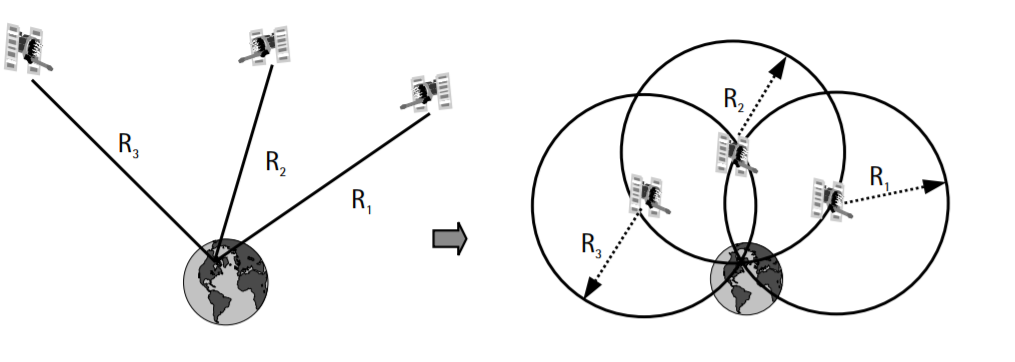
\includegraphics[width=0.8\textwidth]{Images/gps.PNG}\\
    \captionsetup{justification=centering}
    \captionof{figure}{Resection used by the satellites to determine the position \cite{GPS} }
    \label{fig:GPS}
\end{minipage}

Each satellite continuously broadcasts a signal composed of two carriers, two digital codes and a navigation message which contains the coordinates of the satellites as a function of the time. Each space vehicle has atomic clocks to ensure the integrity of the navigation message. The codes and the navigation message gets modulated with the two carrier frequencies.  Figure \ref{fig:modulation} shows the generated signals that are sent from each satellite.

 
 
 \begin{figure}[H]
\centering
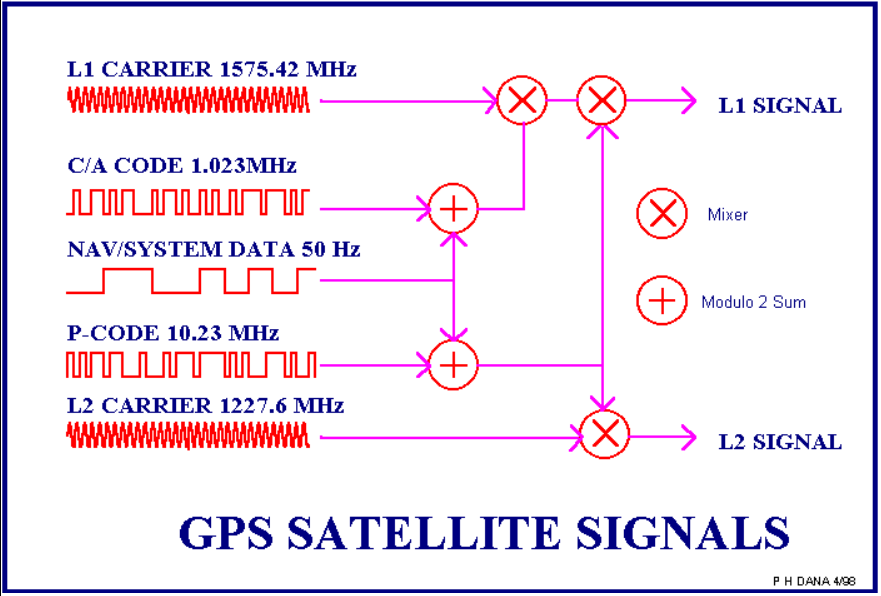
\includegraphics[width=14 cm]{Project_Report/Images/satsignals.PNG}
\caption{The modulation of GPS signals\cite{GPSSIGNALS}}
\label{fig:modulation}
\end{figure}


The two carrier frequencies L1 and L2 that the satellites transmits are generated at 1.5 MHz and 1,2 MHz respectively.  Each SV transmits the L1 and L2 signal but the code modulation for each is different to avoid interference. The two digital code coarse acquisition code (C/A) and precision code(P) consists of a stream of binary digits. The codes are generated using an algorithm and enables a receiver to distinguish the satellites since each have their own set of codes.


The distance between the satellite and the receiver are needed for using the method of resection. The Pseudorange is used for measuring the distance by assuming that the clock of the receiver and satellite are synchronized. The receiver can therefore produce the digital codes at the same time instant the satellites transmits them from space. The distance can be calculated by measuring the difference in delay of the transmitted signal from the produced one. The clocks is not perfectly synchronized, and this is the reason for the name pseudorange.
A method for determining the velocity of a receiver, is by estimating the Doppler frequency of the received signal. The Doppler shift is caused by the relative motion of the receiver and the SV.
 
  
 
 The navigation message contains the Ephemeris, the Almanac, the health of the SV, the clock correction, and the atmospheric data. The Ephemeris is the precise information about the orbital position and clock correction for the specific satellite. The Almanac is a coarse orbital data of all satellites in the constellation. The Ephemeris is only valid for four hours and is sent every 30  seconds, while the Almanac is valid for 180 days and is sent every 12.5 minutes. 
 The control segment of the GPS system consists of a number of world wide positioned tracking stations and a master control station located in the United States. The control segment tracks the satellites to predict their location, control the atomic clock and satellite data that is transmitted by the SV. The user segment consists of GPS receivers that is used to determine their position.
  
  
 \subsection{Acquisition and Tracking}
  
The operation of a GPS receiver consists of two distinct phases: acquisition and tracking. Acquisition is the initial phase after start up. This is where the receiver searches and tries to detect the C/A codes from the satellites. After detecting and receiving satellite data from minimum four satellites, the receiver starts the tracking phase.

After synchronizing the clock, the receiver determines the position and continues to search for other satellites signals during the tracking phase. The receiver switches to the acquisition phase, whenever it doesn't detect minimum four strong satellite signals.
Most receivers uses two separate engines for acquisition and tracking. The acquisition phase is usually the most power demanding of the two. The time to first fix (TTFF) depends on three scenarios:
\begin{itemize}
\item Cold start: This is the same as a factory reset. The receiver doesn't have the last positional fix, the time or any valid satellite data of the constellation. Standard time to first fix  is about 30 \,s - 60 \,s.
\item Warm start: Last position, time and the Almanac is valid. The receiver does only have to download the Ephemeris from the satellites. Standard estimation of TTFF is around 35 \,s - 50 \,s.
\item Hot start: When the previous fix was 1 \,s ago, all the data is valid and the estimated time to next fix is 1 \,s. 

\end{itemize}




\newpage
%%%%Measurment methods for measuring/estimating energy consumption
\chapter{Measurement methods}
As the complexity and energy demand of today's electronics is developing rapidly, it's important to have good models of the energy usage of the devices in the industry. Low-energy design is therefore one of the biggest research topics in today's electronics and has produces numerous methods for measuring, estimating or decreasing the energy consumption of a device. There are several alternatives for modeling the energy consumption of a system, where the main difference is that the energy either gets estimated or measured. The following section will present some of these methods. The quality of the estimation and measurement techniques varies from a 20\% error rate to as low as 0.1\%.  The energy consumption can either be estimated before the execution of the program as in software estimation, or it can be directly measured as with a shunt resistor. The appropriate method to use depends on the system that is under measurement, as some of the methods require detailed knowledge of the system, while other threat the system as a black box.
\section{Shunt resistor}
A shunt resistor is often used to measure the energy consumption of a load because of its cost friendly and simple configuration \cite{Intersil} \cite{Infineon} \cite{Vishay}. The shunt is placed in series with the device and the power supply.

If the voltage drop $V_{shunt}$ is measured, the current I can be calculated by Ohms law:\begin{equation}
V_{shunt}=R_{shunt}*I
\end{equation}

$R_{shunt}$ should be of a small value so it doesn't interfere with the circuit. The power used by the device can then be calculated by using the power relation:
\begin{equation}
P=V_{load}*I \\
\end{equation}
\begin{equation}
V_{load}= V_{supply}-V_{shunt}
\end{equation}

 The resistor value of the shunt should be of a small value to minimize the power dissipated by the shunt. From \cite{Intersil}, we get the relation between temperature coefficient, temperature resistance and resistance value:
\begin{equation}
\Delta R= R_{initial}* \Delta T * T_{coefficient}\\
\label{rchange}
\end{equation}
\begin{equation}
 \Delta T = \theta * I^{2}*R_{sense}
\end{equation}

The temperature change in the shunt comes mainly from the heat of the power dissipation that is caused by the current flowing into it. A smaller package has a higher thermal resistance $\theta$ and therefore a higher resistance change when power dissipation increases. Figure \ref{fig:Powererror} from \cite{Intersil} shows the error of three different shunt resistors with different packages. 

\begin{minipage}[t]{0.8\textwidth}
\centering
    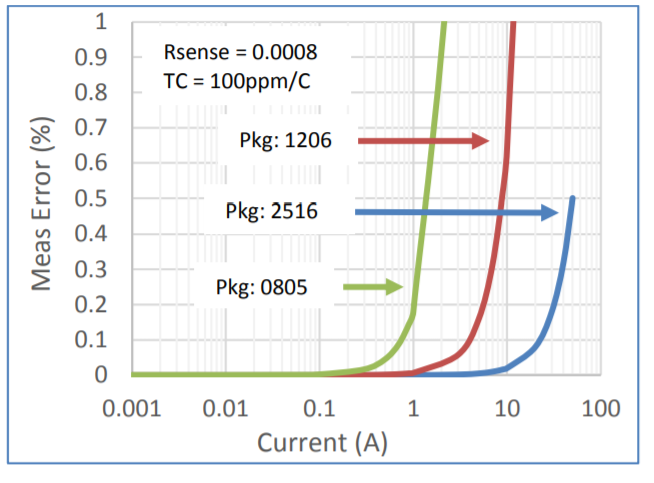
\includegraphics[width=0.8\textwidth]{Images/Powererror.PNG}\\
    \captionsetup{justification=centering}
    \captionof{figure}{The measurement error of 3 shunt resistors with different packages from \cite{Intersil}}
    \label{fig:Powererror}
\end{minipage}


The shunt can be placed either in a high side or low side configuration. A low-side shunt has one of its terminals grounded, this configuration might be preferable as the shunt resistor is not exposed of the high common node voltage that might damage the measurement device. The configuration does also give the measurement device an easy access to common ground, so that more signals can be measured at the same time in reference to a stable ground. A high-side configuration places the shunt between the power supply and the load. This might be preferable because it connects the load directly to the ground of the power supply. This configuration enables the shunt to detect leakages that appear before the load, which may have not been detected by the low-side configuration. Figure \ref{fig:shunt} shows the two configurations. \hfill \break


\begin{figure}[h]
\centering
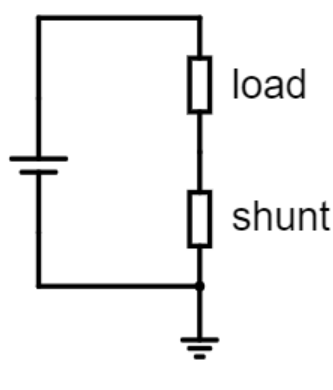
\includegraphics[height=4.5cm]{Project_Report/Images/shunt.PNG}
\caption{The setup for a high-side shunt and a low-side shunt to left and right respectively}
\label{fig:shunt}
\end{figure}




\section{Hall effect}
The Hall effect can be exploited to measure the current in the circuit. When a current $I$ flows in to a conductor it also changes the magnitude of the magnetic field $H$ proportionately. The relation between the flux density $B$ and $I$ can be expressed as follows:


\begin{equation}
B= \mu_{0}*\mu_{r}*H= \frac{\mu{0}*\mu{r}*I}{2\pi r}
\end{equation}

An Hall effect IC consists of a Hall effect sensor which deliver an output signal which is a linear function with the flux density. The IC is a a loss less system because no resistance is inserted into the circuit and therefore a good method of sensing current without interfering the load.  The IC does also require a field concentrator to boost the flux density for the measurement.
\begin{figure}[ht]
\centering
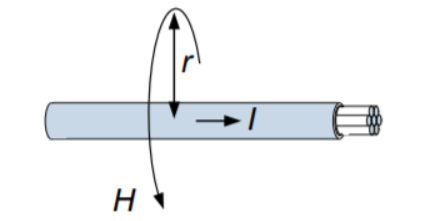
\includegraphics[height=4.5cm]{Project_Report/Images/current.PNG}
\caption{The induced magnetic field of a conductor from \cite{Infineon}}
\label{fig:current}
\end{figure}


\section{Software based estimation}

In \cite{EAC} Kadayif et al presents a framework that can estimate and optimize energy consumption of a high level code. The model is validated by using a cycle-accurate architectural-level energy simulator and is within a 6\% error margin. The input to the framework is its program code, architectural, transistor technology, energy model and the energy constraints. The paper uses a five staged pipeline datapath for the architectural parameter with a 0.35 micro transistor technology. The energy model that the framework uses is the sum of the energy consumed in different components. The components that are used to estimate the energy consumption consist of datapath, bus, main memory, cache and a clock network. Figure \ref{fig:EAC_table} shows the energy-dependent parameters of each component in the energy model and how they can be extracted from the high level code. The energy constraints are only used if optimization of the code is desired. 
\begin{figure}[H]
\centering
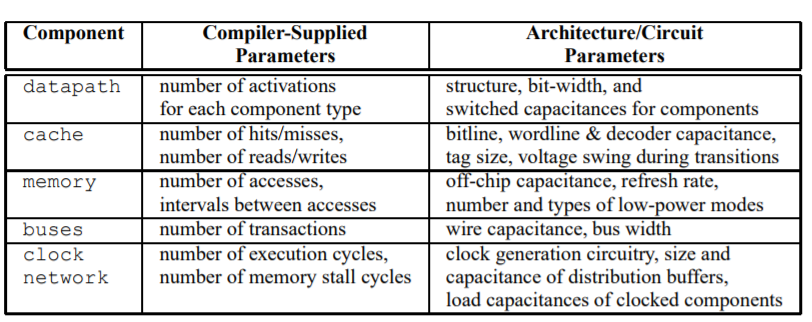
\includegraphics[height=4.5cm]{Project_Report/Images/EAC_table.PNG}
\caption{The energy dependent parameter of each component in the energy model and the belonging parameters in high-level code \cite{EAC}}
\label{fig:EAC_table}
\end{figure}
In \cite{Software_Energy} Deguang et al presents a method for estimating the energy consumption at architecture-level by using an extreme learning machine(ELM).  They model the architecture of the software system as a complex network, where the nodes are the software and the edges between them are the interactions. The energy model they proposed is given by \ref{software equation}

\begin{equation}
 E_{s}= P*T_{s} = f(m_{s})*T_{s}=f(V,E,L,K,C)*T_{s}
\label{software equation}
\end{equation}

$E_{s}$ is the total energy consumption over a $T_{s}$ period. P is the power consumption. $m_{s}$ is the network characteristics and f is the relation between the energy consumption and the network. f depends on the number of nodes V, the number of edges E, average path length L, the clustering coefficient L and the average degree of software network K. By using reverse software engineering they train the ELM to fit the nonlinear correlation function f and uses the ELM to estimate the energy consumption. They compare their model to a pTop model and achieves a 7.9\% error rate. 

\section{Cycle based energy estimation}
 Energy estimation can be done at RTL level by using cycle based energy models. In \cite{Energy_Gupta} Subdoh et al present a macro modeling technique for estimating the energy per cycle for a logic circuit for every input pair vector pair. The paper presents a automatically characterization procedure that can be used to build equation based energy per cycle macro models. The average error of the estimating the energy per cycle is under 20\%. \newline
 
 \cite{Energy_Ana} provides an approach for cycle-accurate hardware/software co-simulations of energy consumption. The simulation framework gets energy estimations for high level descriptions of embedded systems. The energy estimation is obtained by creating energy models for every hardware block and including them in functional models of the "Tool for system simulation"(TSS) simulator. An approach for creating energy models where no structural gate information is known is  presented in the article. 
 
\chapter{Measuring platform}

The method of shunt resistor was chosen to measure the energy consumption of the GPS system. The shunt resistor was chosen due to its low complexity compared to the Hall effect IC.  The other software estimation techniques and cycle aware techniques was not chosen, as they either tries to estimate the energy consumption with poor accuracy or they need non available RTL information about the design. The shunt resistor threats the system that is getting measured as a black box, which enables the measuring platform to be used with any system. Two configurations of the measurement platform with a shunt resistor was developed. This section will explain the functionality of each component of the measurement platfrom.


\section{PicoScope 640 AD}
PicoScope 6000 from Picotecnology is a 4 channel digital oscilloscope with 5GS/s sampling and 2 GSample buffer memory \cite{Pico}. The oscilloscope is equipped with USB 3.0 and supplied with an SDK that enables the user to write their own software. The PicoScope has advanced trigger possibilities and a bandwidth of 500MHz along with a signal generator. The oscilloscope is used to measure the voltage drop across the shunt resistor.   

\section{PC with Python script}
A Python API that uses the SDK from Picoscope is executed on the PC. The script is a modified version of the framework by Amen Hussain \cite{Amen}. The script is included in appendix \ref{Appendix:EnergyMeasure.py}. The script measures the voltage drop over the shunt resistor by using the following parameters:

\begin{itemize}
    \item sampling- The sampling frequency 
    \item duration- The length of each waveform
    
\end{itemize}
The sampling and duration is used to generate a waveform of the sampled data.
The sequence diagram in figure \ref{fig:sequence} shows the interaction between the python script and the oscilloscope.  

\begin{figure}[H]
\centering
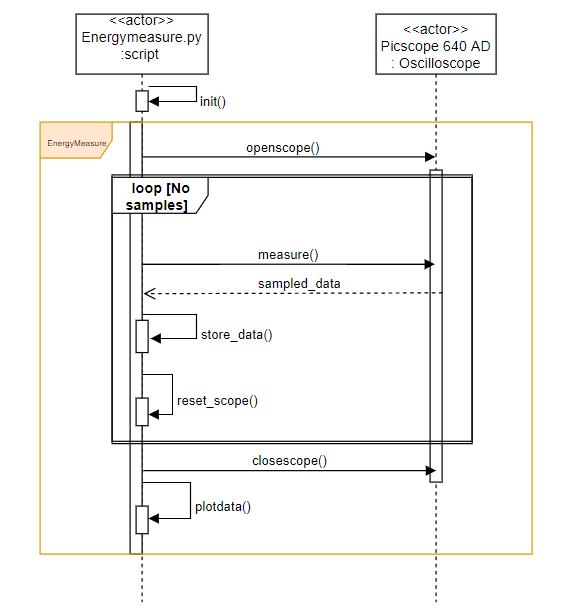
\includegraphics[height=10.5cm]{Project_Report/Images/Sequence_diagram.PNG}
\caption{Sequence diagram for the measurement script}
\label{fig:sequence}
\end{figure}
 

 The script samples the data and stores it in a list, before it restarts the sampling for the next waveform. An overhead of storing data and initializing the oscilloscope before each sample introduces a limit for the processing speed of the measurements. The measured delay caused by the overhead in software is 20-50 milliseconds between each waveform. The delay is found by using timers in software during the execution of the python script. This means that some data is not captured during the overhead process and constrains the accuracy of the measurements.
The Python script generates a plot of each waveform after the data has been analyzed, this is shown in figure \ref{fig:pythonwaveform}

\begin{figure}[H]
\hspace*{-3cm}
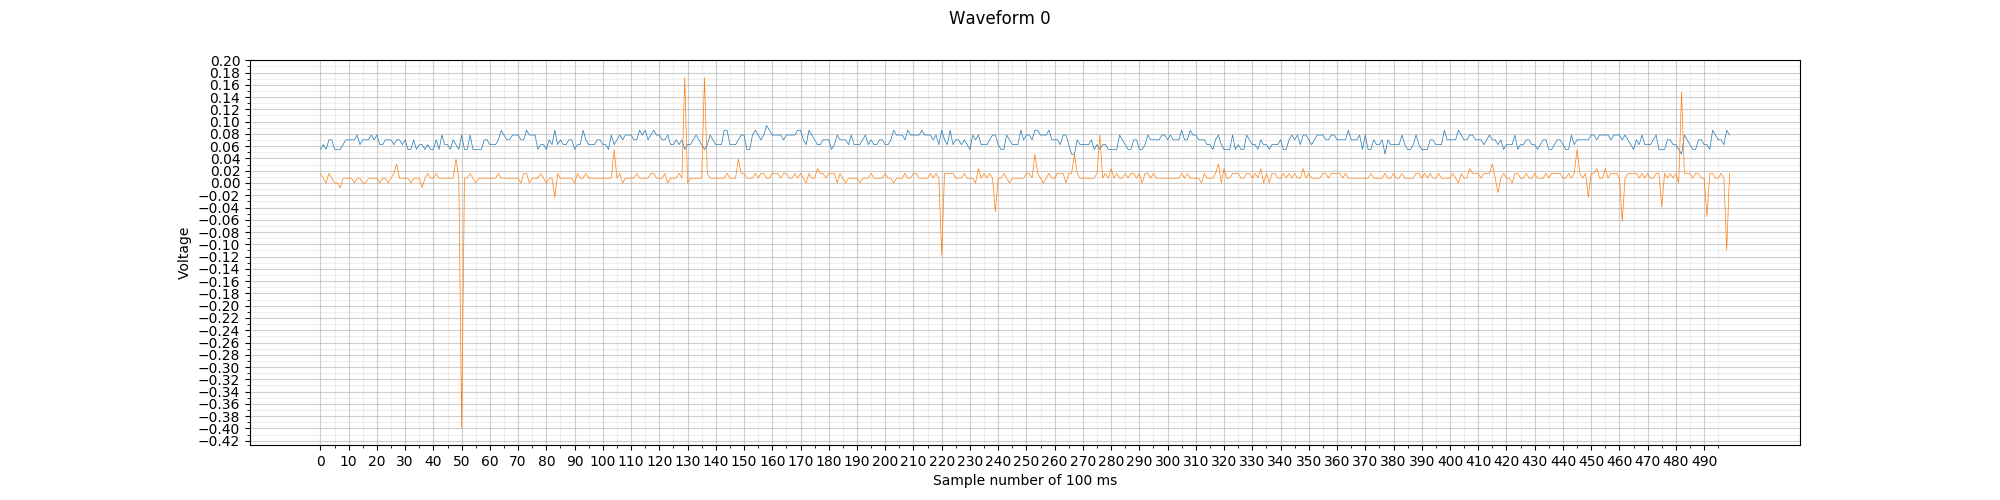
\includegraphics[height=5.5cm]{Project_Report/Images/pythonwaveform.png}
\caption{The waveform that is plotted by the python script and used for analyzing the current consumption}
\label{fig:pythonwaveform}
\end{figure}
 
An Excel document with the average current and power of each waveform is also generated. Figure \ref{fig:waveexcel} shows a screenshot of the generated excel spreadsheet for 13 waveforms.

\begin{figure}[H]
\centering
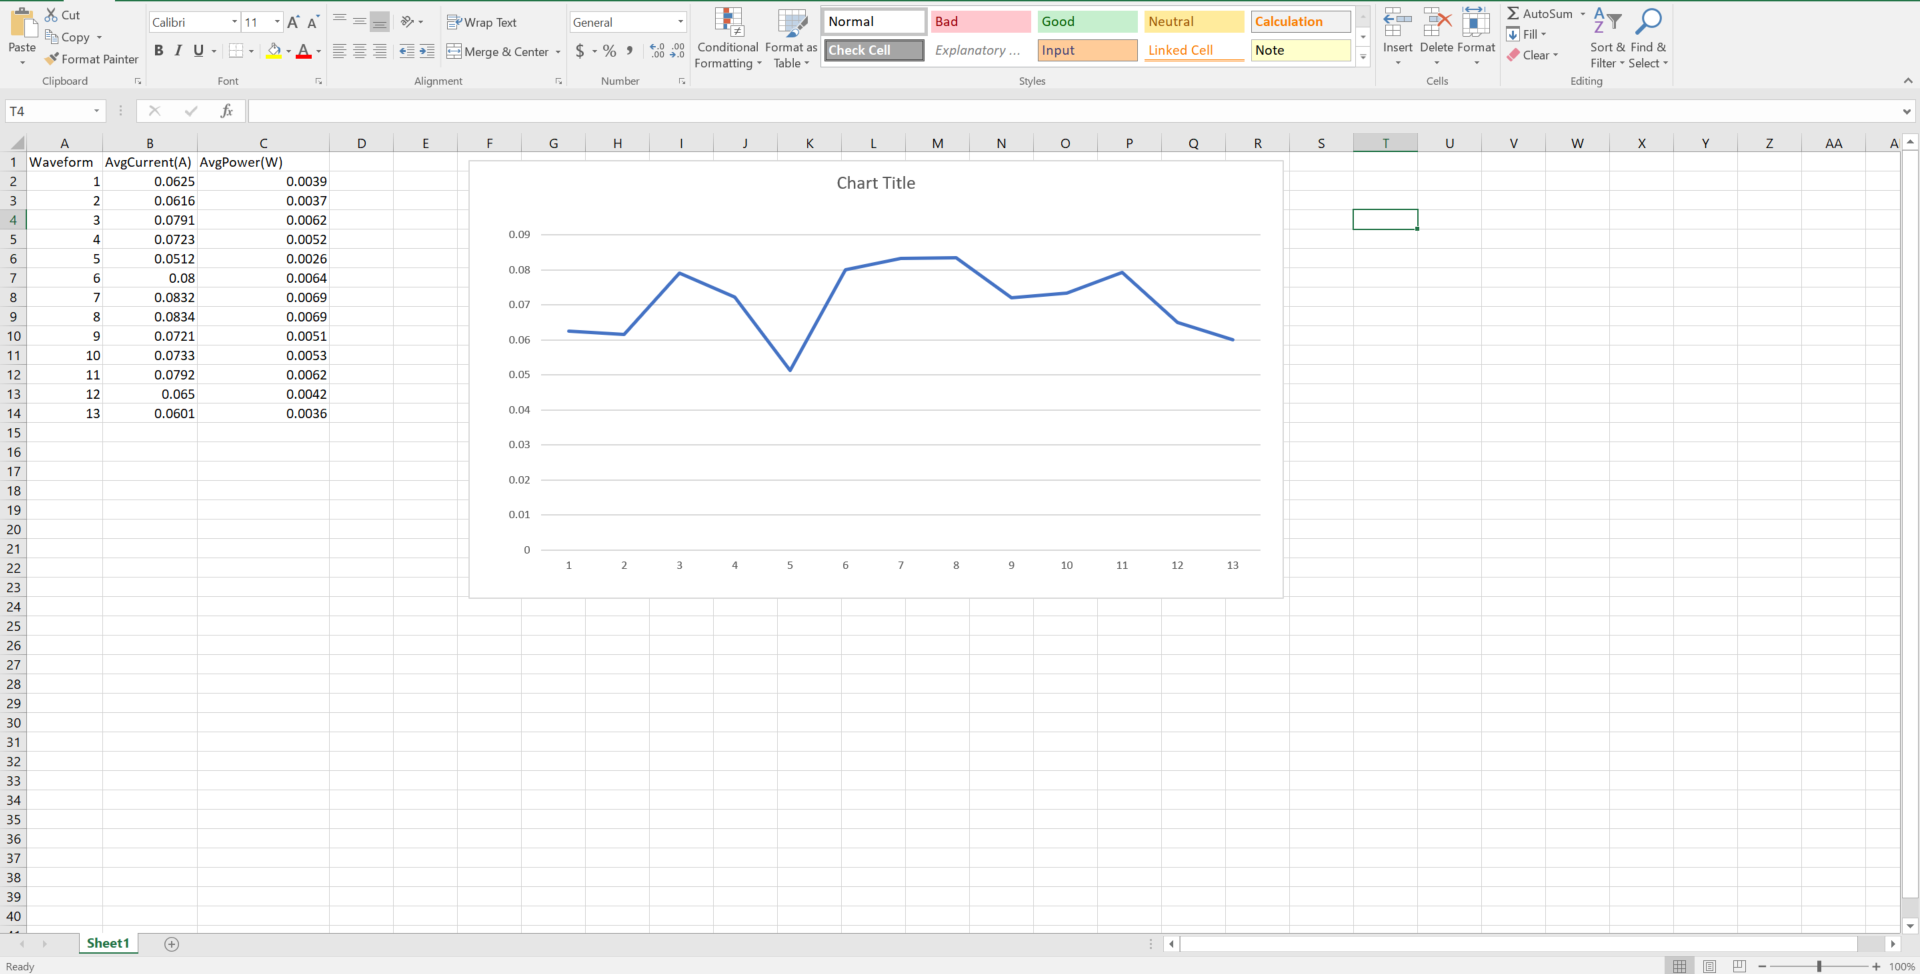
\includegraphics[height=8.0cm]{Project_Report/Images/waveformexcel.PNG}
\caption{Spreedsheet with the average current of 13 waveforms}
\label{fig:waveexcel}
\end{figure}
 



\section{Configuration options}
 Two configurations of the measurement platform with shunt resistor was developed. The first used a C027 application board from u-blox, while the other used a LoPy microcontroller from PyCom. Both methods used the PC and the Oscilloscope. 
 


\subsection{Configuration with C027}
Figure \ref{fig:deploy_C027} shows the deployment diagram of the configuration with the C027 development kit.  

\begin{figure}[H]
\centering
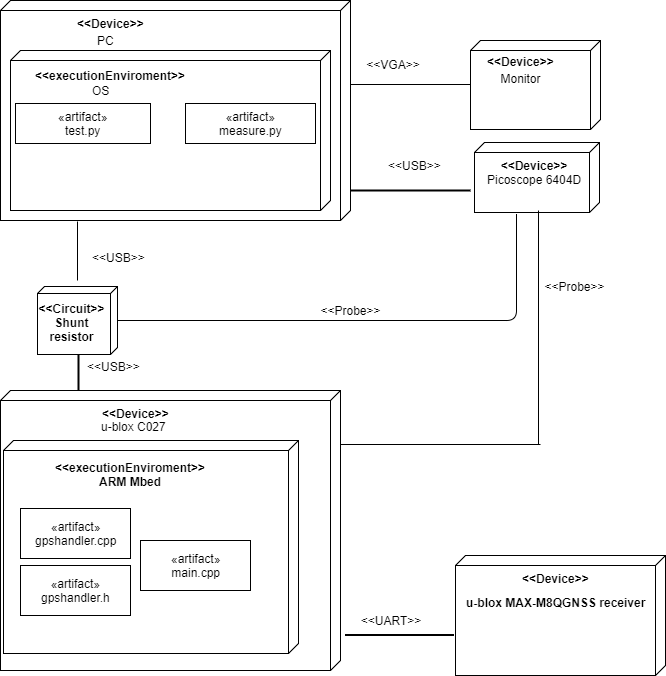
\includegraphics[height=9.5cm]{Project_Report/Images/C027_deploy.png}
\caption{Deployment diagram of the configuration with the C027}
\label{fig:deploy_C027}
\end{figure}
\vspace{5mm}The u-blox C027 is a development board for IoT applications that supports GSM, UMTS and CDMA networks. The development board has a MAX-M8Q GNSS receiver and a cellular module. The header connector has 6 analog inputs, 9 PWM, 22 GPIO, 1 SPI, 1 I2C, 1 UART and 1 I2S. C027 is supported by ARM Mbed, which is an operating system for IoT devices \cite{C027}. The application board has no embedded low power mode, but some peripherals like the GPS can be turned off with UART. Time to first fix (TTFF) for the receiver is \cite{MAX-M8}:
\begin{itemize}
    \item Cold start: 30 \,s
    \item Hot  start: 1 \,s
\end{itemize}

Two threads are run in "main.cpp" on the C027, the first thread receives the requested command from the PC and updates a shared variable between the two threads. The value of the shared variable corresponds to a predefined action. The second thread checks the value of the shared variable and executes the action by sending a certain sequence of bits over UART to the GPS. At the same time the action is executed, a GPIO pin is pulled high to signalize to the PC that a measurement should be done. The code that was written for C027 is included in the appendix \ref{Appendix:C027.Cpp}. 

To measure the current consumption of the application board, we had to put the shunt resistor between the VCC and GND from the USB connection. The VCC for the USB connection could not be sourced from the USB port because the value of the VCC would not be constant 5v and therefore introduce an error to the measurement. We decided therefore to use a 12 V battery and the LM317 voltage regulator for producing the VCC for the application board. Figure \ref{fig:Schematic_C027} shows the schematic of the C027 configuration with the LM317 voltage regulator. 

\begin{figure}[H]
\centering
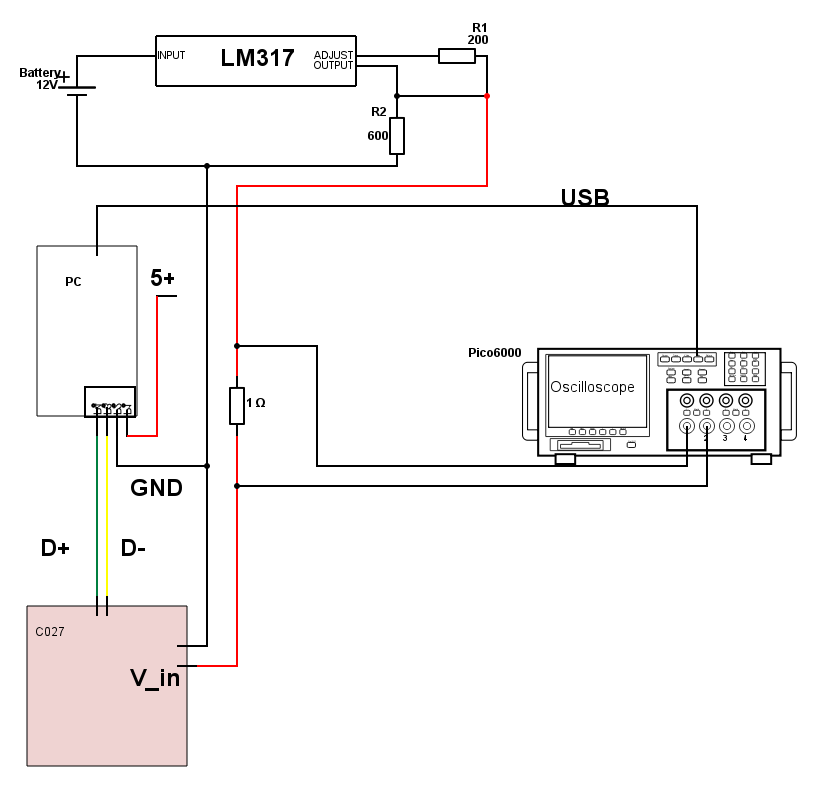
\includegraphics[height=8.5cm]{Project_Report/Images/C027_Schematic.png}
\caption{Schematic of the C027 configuration}
\label{fig:Schematic_C027}
\end{figure}

The oscilloscope measures the voltage after the shunt resistor. The voltage drop over the shunt resistor is estimated by first measuring the output of the voltage regulator, and then measuring the voltage after the shunt resistor and subtracting them in software. Measuring the voltage drop directly will change the common ground for the oscilloscope, C027 and the PC to the node after the shunt resistor. This is undesired, because it prevents the oscilloscope from measuring another signal which is not referenced to that GND. 

Difficult debugging, short circuiting of the PC and a too complex configuration encouraged us to develop another simpler measurement platform. 



\subsection{Configuration with LoPy}
Another option for the measurement platform was a circuit with the LoPy microcontroller from Pycom. An overview over the measurement platform is shown in \ref{fig:LoPy_deploy}. 

\begin{figure}[H]
\centering
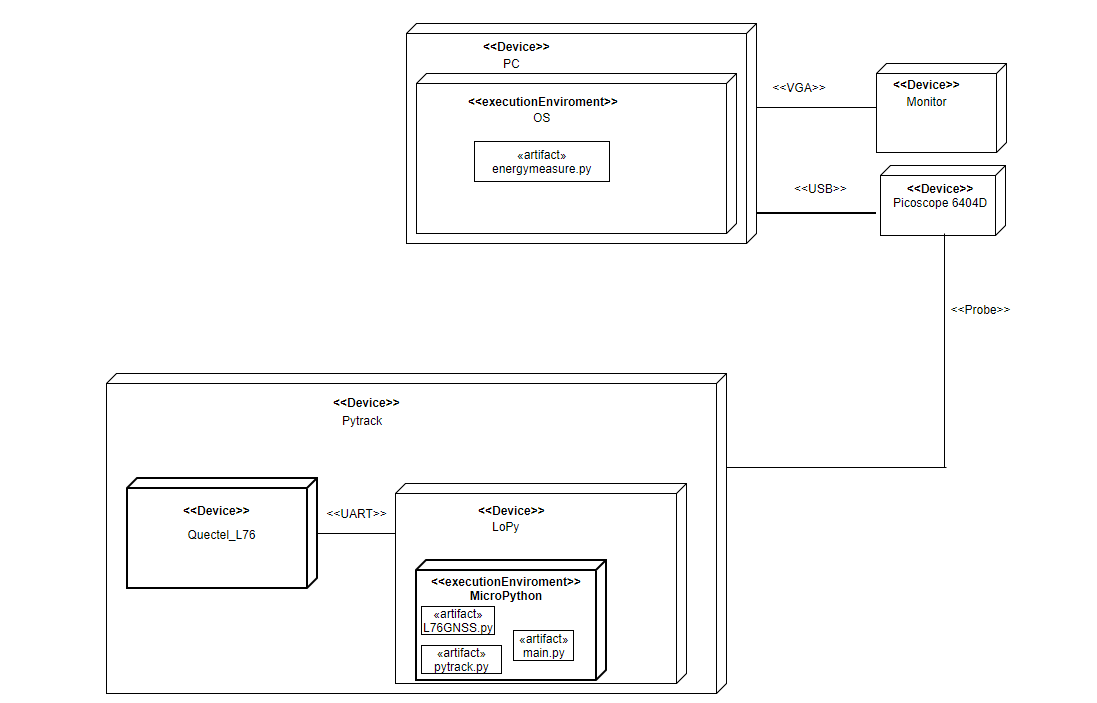
\includegraphics[height=9.5cm]{Project_Report/Images/LoPy_deploy.png}
\caption{Deployment diagram of the LoPy configuration}
\label{fig:LoPy_deploy}
\end{figure}

The LoPy is a microcontroller equipped with a LoRa, Wifi and BLE technology \cite{LoPy} and is specifically made for IoT use cases. It uses the Espressif ESP32 chip and the user write the program code in MicroPython. LoPy has a low-power feature which makes it turn off most of the hardware except its internal peripheral. The micro controller has UART, SPI, I2C and up to 24 GPIO.

The LoPy is equipped with Pycom's Pytrack, which is an extension shield to the LoPy. Pytrack is equipped with a L76-l GPS receiver from Quectel and a 3 axis 12 bit 
accelerometer \cite{Pytrack}. L76-l is a low power GNSS receiver \cite{L76}. The module is equipped with an ARM7 processor and UART for serial communication. The LoPy controls the receiver through the execution of the program code and communicates with the ARM7 processor through serial communication with the Pytrack shield. TTFF for the GNSS receiver is:
\begin{itemize}
\item Cold start:35 \,s
\item Warm start: 30 \,s
\item Hot start: 1 \,s


\end{itemize}


The LoPy offers debugging possibilities over WiFI which enables a simple configuration by measuring the voltage drop directly over the shunt resistor. The schematic of the circuit configuration is shown in \ref{fig:LoPy_Schematic}. The green channel is the common ground for both the red channel and the black channel. The red channel measures the voltage drop over the shunt. The measured signal is inverted in software because it's referenced to a node that has a higher potential. 

\begin{figure}[H]
\centering
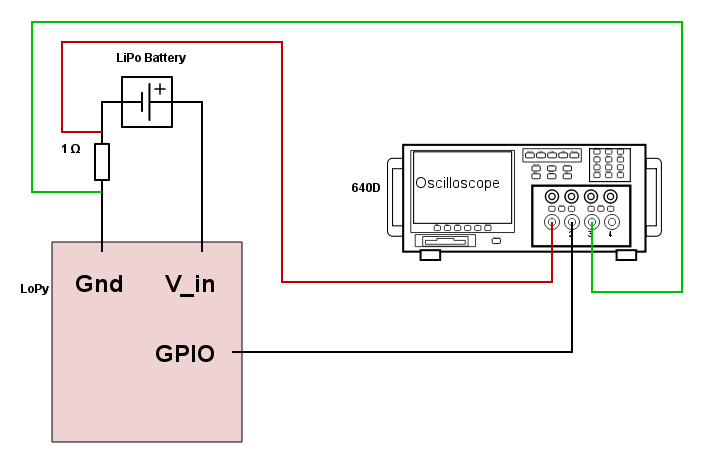
\includegraphics[height=6.5cm]{Project_Report/Images/LoPy_Schematic.png}
\caption{A low side shunt configuration}
\label{fig:LoPy_Schematic}
\end{figure}


\subsubsection{Program code for acquiring a positional fix}
Program code is written for the LoPy. The code is based on the framework published from PyCom. The code initializes the serial communication with the ARM microcontroller on the Quectel L76-l receiver. The next step is to parse the satellite data that is sent from the receiver to the LoPy. The data is sent according to the NMAE protocol. A part of the program code is shown in \ref{code:Parsing of gpsdata}. The code reads the data from serial and tries to find the GPGGA data. The GPGGA contains the fix status and other satellite data. If the GPGGA data is found, the fix status is read and set. The remaining code is included in the appendix \ref{Appendix:L76GNSS.py}

\lstset{language=Python}          % Set your language (you can change the language for each code-block optionally)

\begin{lstlisting}[frame=single]  % Start your code-block

            nmea += self._read().lstrip(b'\n\n')
            .rstrip(b'\n\n')
            gpgga_idx = nmea.find(b'GPGGA')
            if gpgga_idx >= 0:
                gpgga = nmea[gpgga_idx:]
                e_idx = gpgga.find(b'\r\n')
                if e_idx >= 0:
                    try:
                        gpgga = gpgga[:e_idx].decode('ascii')
                        print (gpgga)
                        self.gpgga_s = gpgga.split(',')
                        print(self.gpgga_s)
                        self.get_fix()
                        if(self.fix >0):
                            self.lat_d, self.lon_d
                            = self._convert_coords
                            (self.gpgga_s)
\end{lstlisting}
\label{code:Parsing of gpsdata}









.
\newpage
%\begin{table}[h!]
%\begin{center}
 %\begin{tabular}{||c c c c||} 
 %\hline
 %Waveform & AvgCurrentA(A) & Power(W) & AvgCurrentB(A) \\ [0.5ex] 
 %\hline\hline
 %4827 & 0.0831 & 0.0069 & 0 \\
 %\hline
 %4828 & 0.0822 & 0.0067 & 0 \\
 %\hline
 %4829 & 0.0833 & 0.0069 & 0 \\
 %\hline
 %4830 & 0.0822 & 0.0067 & 0 \\
 %\hline
 %4831 & 0.0796 & 0.0063 & 0 \\ 
 %\hline
 %4832 & 0.0830 & 0.0069 & 0 \\
 %\hline
 %\rowcolor{red}
 %4833 & 0.0759  & 0.0057 & 3.3 \\[1ex]
 %\hline
%\end{tabular}
%\end{center}
%\caption{The table shows the data when a positional fix is acquired.}
%\label{Table:wifioff}
%\end{table}



\chapter{Measurements}

 This chapter presents the results and the program code that was used during the  specific test. The first step was to measure the current consumption of the LoPy during a request of positional fix. Measuring of data was done outside with the measurement platform. All the measurements was done under similar weather conditions. 


\section{Measurement with communication}
Program code for getting a positional fix is shown in \ref{code:intial}. The program initialize a GPIO pin that is toggled when a positional fix is acquired. The function coordinates() is from the L76 GNSS class, and sets the class variable fix when the position is received. 
\lstset{language=Python}          % Set your language (you can change the language for each code-block optionally)
\begin{lstlisting}[frame=single,caption = main.py]  % Start your code-block

#intialize the trigger output and the Pytrack/GPS
p_out = Pin('P20', mode=Pin.OUT)
p_out.value(0)
py = Pytrack()
l76 = L76GNSS(py)
while (True):
    #Toggle the trigger when a fix acquried
    coord = l76.coordinates()
    print ("FIX: ", l76.fix)
    if ((l76.fix) and not(l76.first_fix)):
        l76.first_fix = 1
        l76._set_time()

        p_out.value(1)
        time.sleep(0.25)
        p_out.value(0)
\end{lstlisting}
\label{code:intial}
After doing some measurements with the program code and analyzing it, it became evident that another power demanding task was running on the LoPy besides the GPS function. The current and power consumption of the 9 first waveforms are shown in table \ref{Table:WIFI_ON}.
\begin{table}[h!]
\begin{center}
 \begin{tabular}{||c c c||} 
 \hline
 Waveform & Avg Current(A) & Power(W)\\ [0.5ex] 
 \hline\hline
 1 & 0.1433    & 0.4523 \\ 
 \hline
 2 & 0.1421    & 0.4487 \\
 \hline
 3 & 0.1365  & 0.4318 \\
 \hline
 4 & 0.1334  & 0.4224 \\
 \hline
 5 & 0.1399  & 0.4420 \\ 
 \hline
 \rowcolor{red}
 6 & 0.1439    & 0.4541 \\ 
 \hline
 7 & 0.1347  & 0.4263 \\
 \hline
 8 & 0.1358  & 0.4296 \\
 \hline
 9 & 0.1358    & 0.4296 \\[1ex]
 \hline
\end{tabular}
\end{center}
\caption{The 9 waveforms after the initial startup sequence}
\label{Table:WIFI_ON}
\end{table}

The row highlighted in red, is the waveform with the highest average current and power consumption.
Figure \ref{fig:startup_intial} shows the plot of waveform 6 that is generated with \ref{fig:sequence}.


\begin{figure}[H]
\hspace*{-3cm}
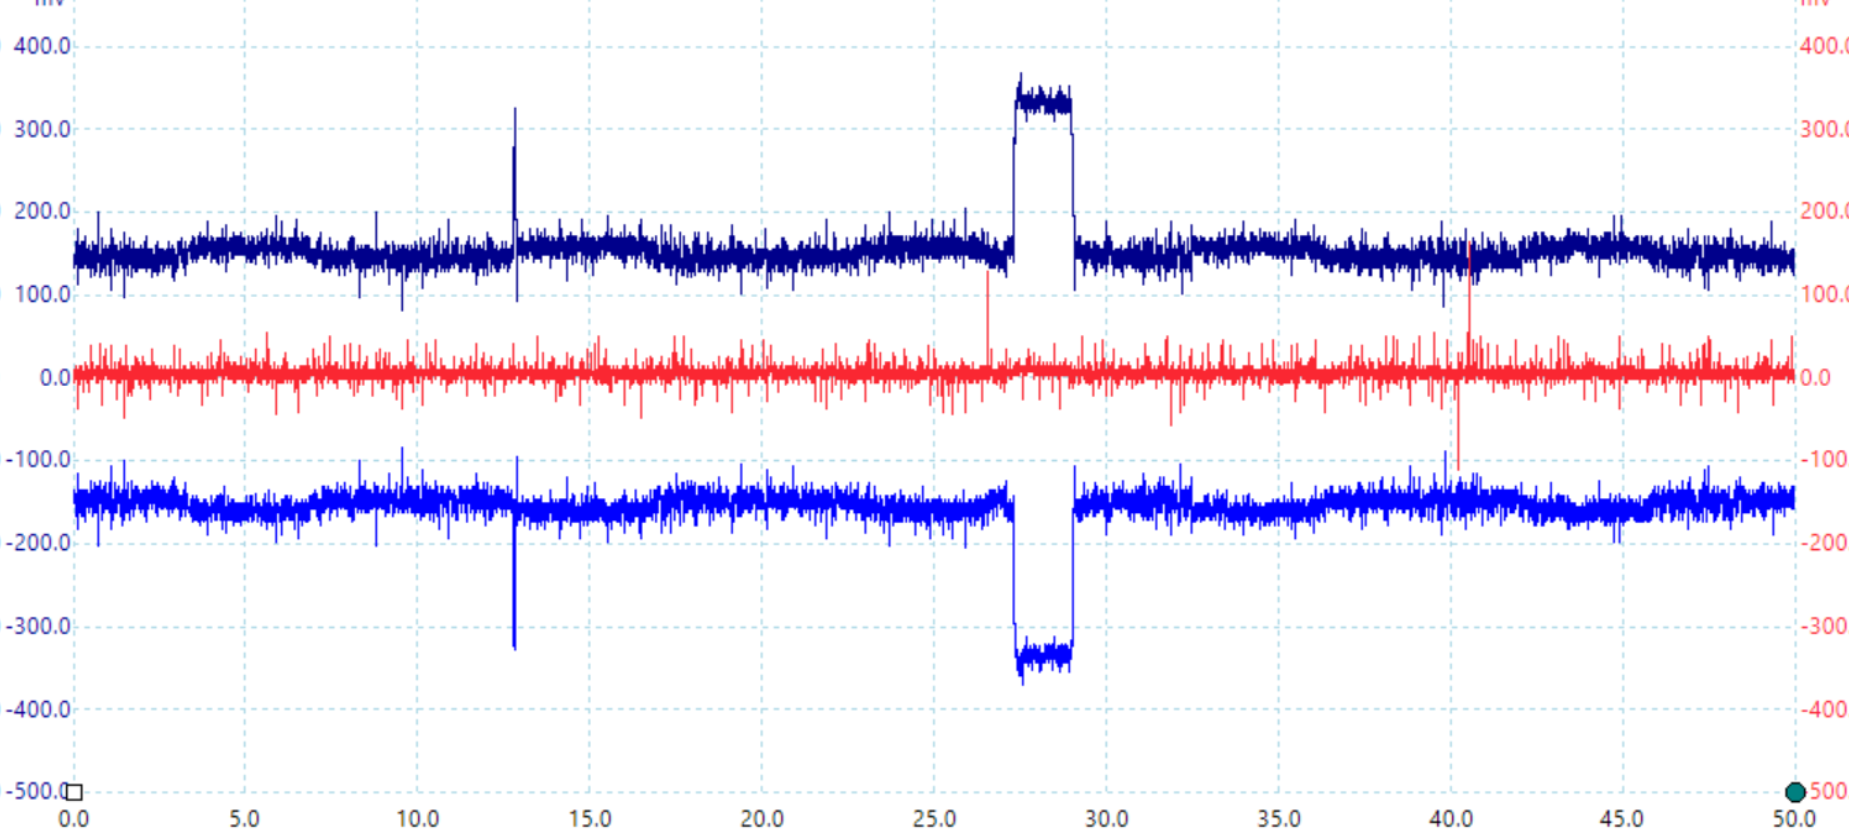
\includegraphics[width=22 cm]{Project_Report/Images/startup_intial.PNG}
\caption{Waveform 6 with the voltage drop(blue) and trigger(orange)}
\label{fig:startup_intial}
\end{figure}

 The conversion of the measured voltage to current is 1:1, since a 1 Ohm resistor is used. The signal have an periodic surge around 430 mA. There are 100 samples between each pulse. A sampling frequency of 5000 S/s gives a sampling interval:
 \begin{equation}
     p= \frac{1}{f} = \frac{1}{5000S/s}= 0.0002 \,s = 0.2 \,ms 
 \end{equation}
 
 The period of the pulse with a sampling period of 0.2 ms and 100 samples between is:
 
 \begin{equation}
     p_{pulse} = 100*0.2 \,ms = 20 \,ms
 \end{equation}
 The measured voltage drop over the shunt resistor is subtracted from the voltage supply of 3.3 \,V to get the voltage drop over the LoPy.
 After reviewing the results, it becomes obvious that the high average current is due to the disturbance from the periodic signal. The periodic signal makes it difficult to relate the power consumption to the GPS, as it influences the current consumption.


\section{Measurement without communication}

The periodic signal is understood as the communication protocol of the Wi-Fi and Bluetooth. The first part of the improved program code, turns the wireless protocols off to remove the disturbance. A COLD START is sent to the ARM processor to reset the GPS between each execution to remove all satellite data. A deepsleep is included after a positional fix has been acquired. The LoPy restarts the program code after waking up from deepsleep. Figure \ref{code:wifioff} shows the programcode.

\lstset{language=Python}          % Set your language (you can change the language for each code-block optionally)
\begin{lstlisting}[frame=single, caption= main.py without communication]  % Start your code-block

# initialize ``P9`` in gpio mode and make it an output
p_out = Pin('P20', mode=Pin.OUT)
p_out.value(0)
wlan= WLAN()
wlan.deinit()
bt = Bluetooth()
bt.deinit()

py = Pytrack()
l76 = L76GNSS(py

py.setup_sleep(2)
l76.write_gps(l76.COLD_START,False)
time.sleep(2)

p_out.value(1)
time.sleep(2)
p_out.value(0)

while (True):
    coord = l76.coordinates()
    print ("FIX:jared ", l76.fix)
    if ((l76.fix) and not(l76.first_fix)):
        l76.first_fix = 1
        l76._set_time()

        p_out.value(1)
        time.sleep(0.25)
        p_out.value(0)
        py.go_to_sleep(True):
\end{lstlisting}
\label{code:wifioff}

Table \ref{Table:wifioff} shows the average current, average power and the average current of the trigger signal B, when a positional fix is acquired. The row that is highlighted in red shows the transition from acquisition phase to tracking phase. 14000 waveforms was sampled during the test run of the program code. A test run lasted for 1 hour.  


\begin{table}[h!]
\begin{center}
 \begin{tabular}{||c c c c||} 
 \hline
 Waveform & AvgCurrentA(A) & Power(W) & AvgCurrentB(A) \\ [0.5ex] 
 \hline\hline
 4827 & 0.0831 & 0.2673 & 0 \\
 \hline
 4828 & 0.0822 & 0.2645 & 0 \\
 \hline
 4829 & 0.0833 & 0.2679 & 0 \\
 \hline
 4830 & 0.0822 & 0.2645 & 0 \\
 \hline
 4831 & 0.0796 & 0.2563 & 0 \\ 
 \hline
 4832 & 0.0830 & 0.2670 & 0 \\
 \hline
 \rowcolor{red}
 4833 & 0.0759  & 0.2447 & 3.3 \\[1ex]
 \hline
\end{tabular}
\end{center}
\caption{The table shows the data when a positional fix is acquired.}
\label{Table:wifioff}
\end{table}

 Plot \ref{fig:4832} shows that the trigger signal B is low, which means that the receiver hasn't acquired a positional fix. The average current for the waveform is 0.0830 \,A. Plot \ref{fig:4833} shows waveform 4833. The average current is 0.0759 and the trigger signal is high. This means that the receiver has acquired a positional fix and is in the tracking phase. 
\begin{figure}[H]
\hspace*{-3cm}
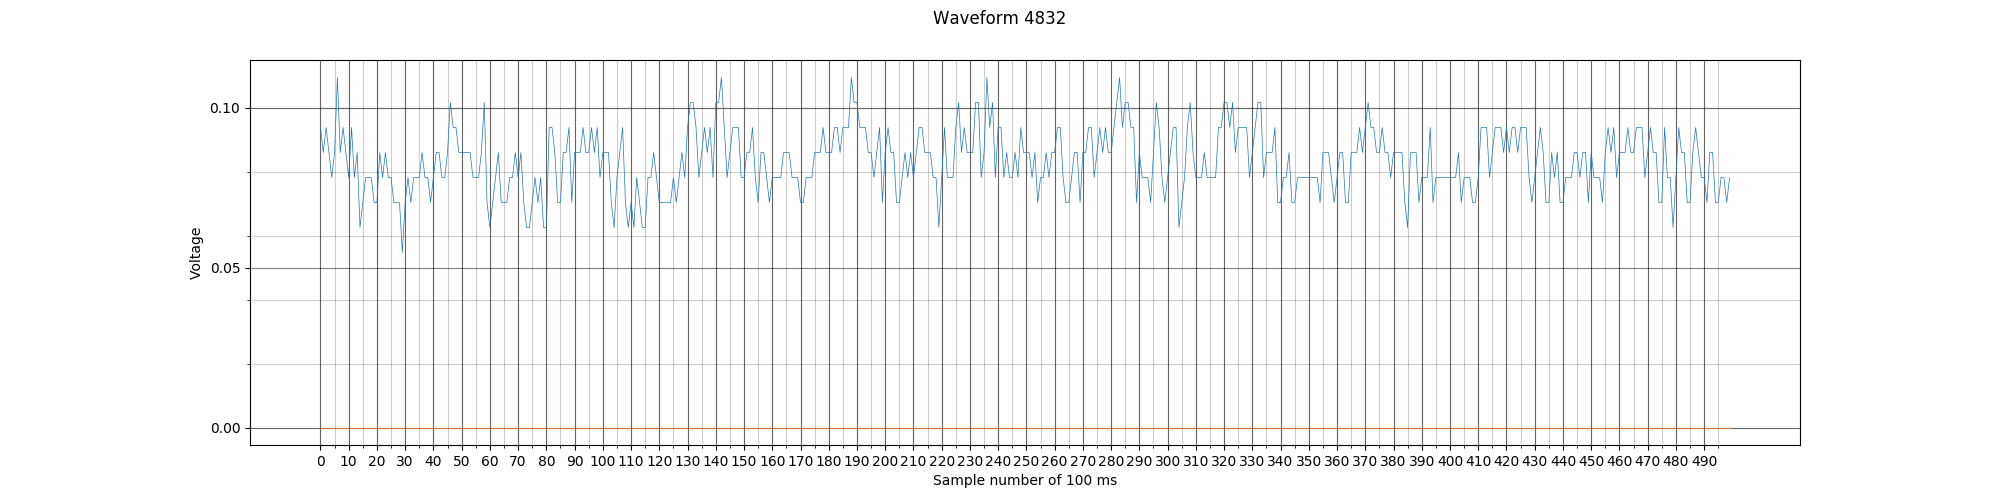
\includegraphics[width=20 cm]{Project_Report/Images/4832.png}
\caption{Waveform 4832 right before a positional fix is acquired}
\label{fig:4832}
\end{figure}

\begin{figure}[H]
\hspace*{-3cm}
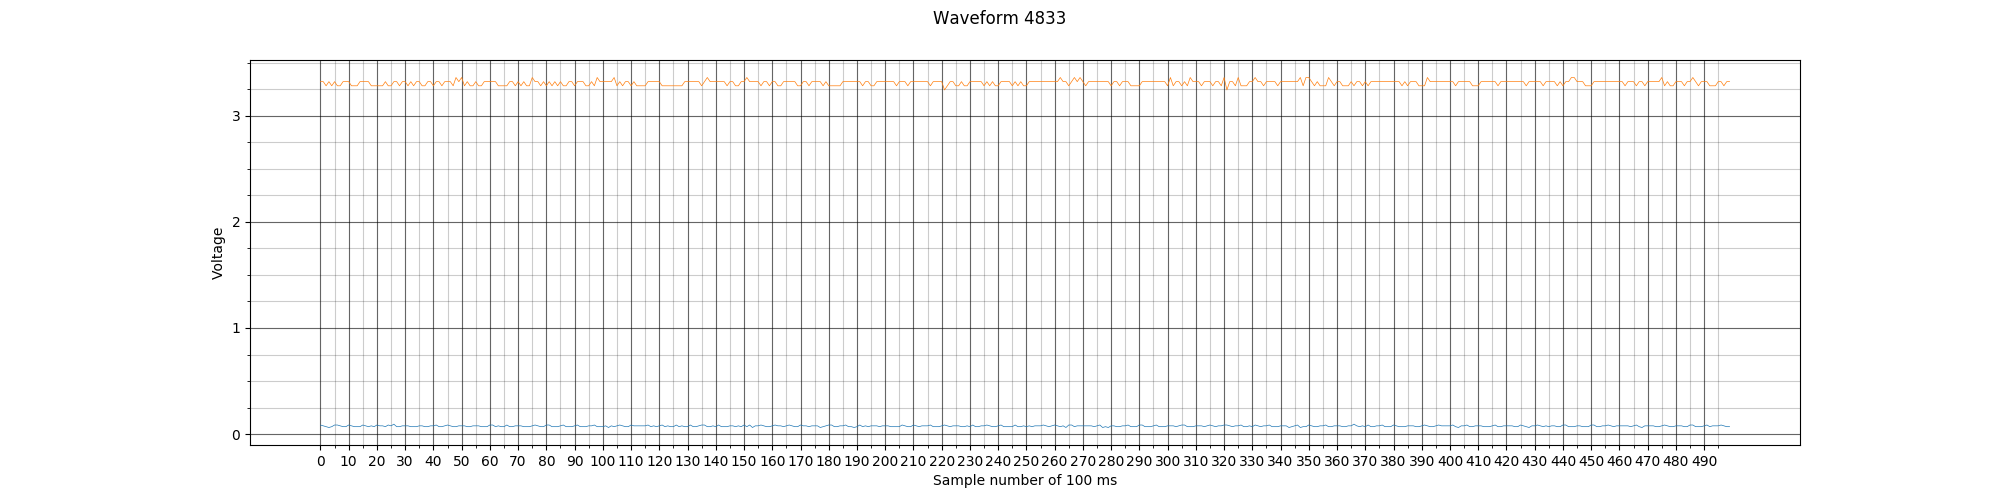
\includegraphics[width=20 cm]{Project_Report/Images/4833.png}
\caption{The waveform when a fix is acquired and the trigger is set}
\label{fig:4833}
\end{figure}




\section{Measuring of deep sleep}
The time from waking up the LoPy from deepsleep until it's searching for signals in the acquisition phase is estimated. The program code used for testing is shown in \ref{code:deepsleep}

\lstset{language=Python}          % Set your language (you can change the language for each code-block optionally)
\begin{lstlisting}[frame=single,caption = main.py for deepsleep measurement]  % Start your code-block

# initialize ``P9`` in gpio mode and make it an output
p_out = Pin('P20', mode=Pin.OUT)
p_out.value(0)

wlan= WLAN()
wlan.deinit()
bt = Bluetooth()
bt.deinit()
py = Pytrack()
l76 = L76GNSS(py)
py.setup_sleep(5)
py.go_to_sleep(True)
l76.write_gps(l76.COLD_START,False)
time.sleep(2)
p_out.value(1)
time.sleep(2)
p_out.value(0)
print("after init")
while (True):
    coord = l76.coordinates()
    print ("FIX:", l76.fix)
    p_out.value(1)
    time.sleep(2)
    p_out.value(0)
    py.go_to_sleep(True)
    if ((l76.fix) and not(l76.first_fix)):
        l76.first_fix = 1
        l76._set_time()

        p_out.value(1)
        time.sleep(0.25)
        p_out.value(0)
\end{lstlisting}
\label{code:deepsleep}


The time is estimated by counting the number of waveforms of 100 ms that is sampled before the initializing sequence signals appears. This time is added together with the overhead of sampling data between each waveform. 42 waveforms is sampled before the initializing sequence appears. 
\begin{equation}
100 \,ms * 42 = 4.2 \,s
\end{equation}
\begin{equation}
3.8 \,s + (20 \,ms*42) = 5.04 \,s \approx  5 \,s
\end{equation}

The average current in deep sleep is measured to 3.2 \,mA. The average current during the initializing sequence is 101 \,mA. 







\newpage
 \chapter{Energy Model}
 To optimally use the GPS receiver, we need an model that can predict the energy consumption of the system. In the first subsection, we will first analyze the data from the measurements. In the next subsection, we will present a parameter exploration for the energy model and finally, we will present the model. 
 \section{Data analysis}
 The first step in making an energy model of the GPS receiver is to analyze the data from the measurements and relating it to the theory. The theory section explains how the receiver operates between two distinct phases: acquisition and tracking. The two phases for a receiver can be modelled in a state diagram. 
 
 
\begin{figure}[H]
\centering
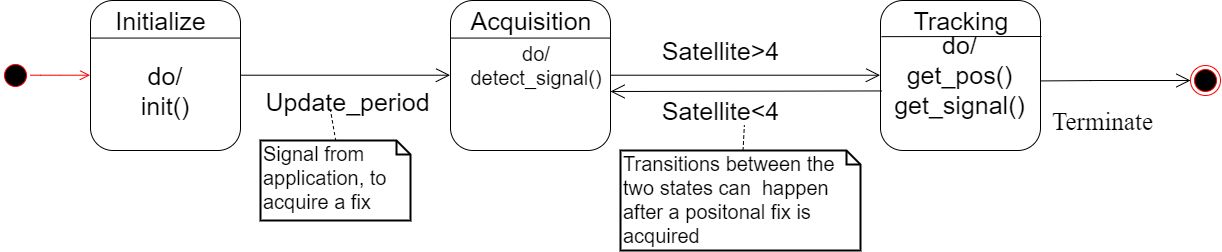
\includegraphics[width=16 cm]{Project_Report/Images/Basic_state_GPS.png}
\caption{The state diagram of a GPS receiver}
\label{fig:GPS reciever}
\end{figure}
The receiver will transition to the acquisition state once the update period is set. It will transition from the acquisition state to tracking state once it has acquired a signal from at least four satellites. 
The trigger functionality from table \ref{Table:wifioff} highlights when the receiver has a positional fix. We know from the theory, that the receiver switches to the tracking phase, once it has acquired a positional fix. The GPS receiver is therefore in tracking phase the instant the trigger is set. The trigger functionality can't however, inform about later transitions because the receiver changes phases after it has a positional fix to maintain the signal strength. A table with the data of the current consumption right before and after the trigger is set, is generated in an acquisition and a tracking column respectively. The average of each phase is calculated.  Average value of the two phases are:
\begin{itemize}
    \item Acquisition state: 80 \,mA
    \item Tracking state: 72 \,mA
\end{itemize}


Figure \ref{fig:averageacq} shows the scatter plot of the average current consumption during the acquisition phase. 
 
\begin{figure}[H]
\centering
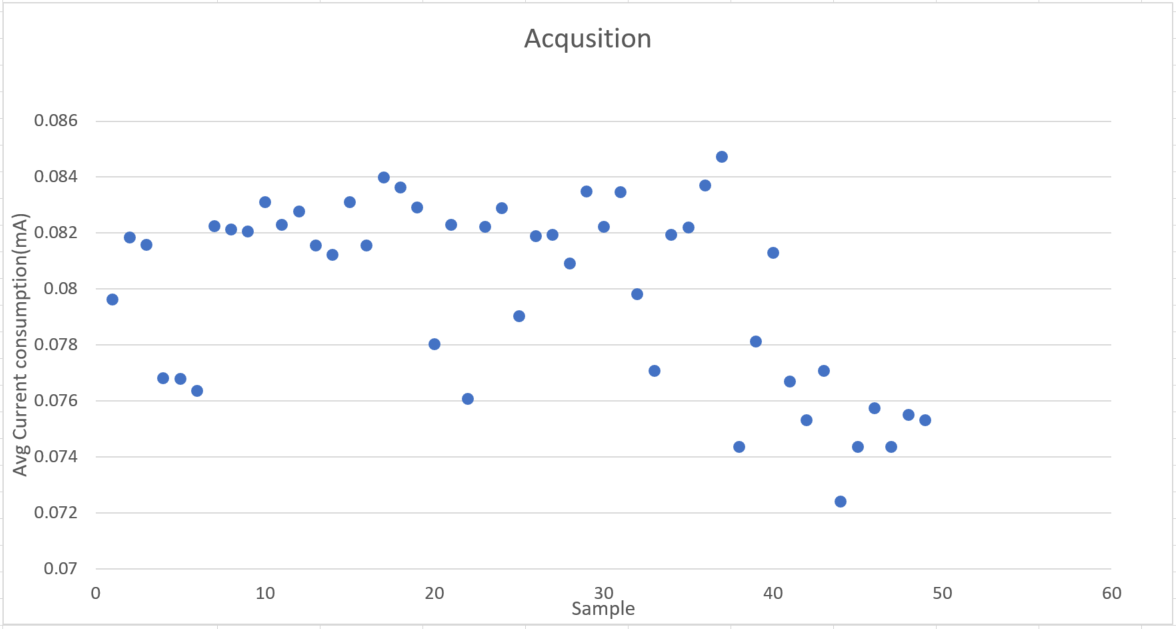
\includegraphics[width=15 cm]{Project_Report/Images/AcqusitionData.PNG}
\caption{The average values for acquisition phase in a scatter plot }
\label{fig:averageacq}
\end{figure}

Figure \ref{fig:averagetrack} shows the scatter plot of the average current consumption during the tracking phase.

\begin{figure}[H]
\centering
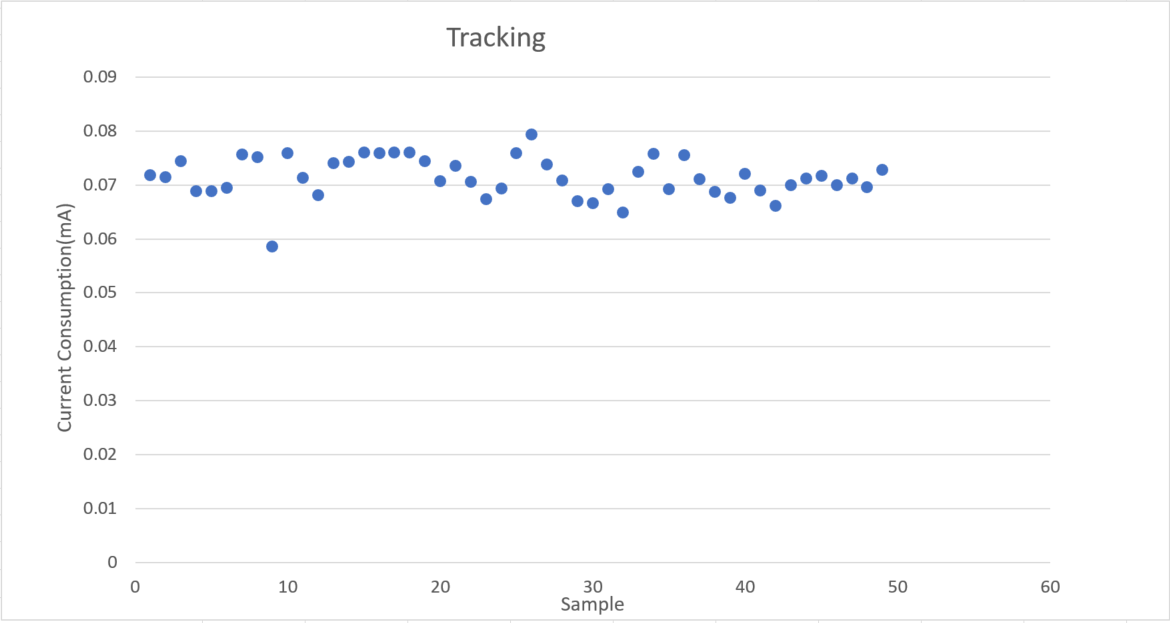
\includegraphics[width=15 cm]{Project_Report/Images/trackingData.PNG}
\caption{The average values for tracking phase in a scatter plot }
\label{fig:averagetrack}
\end{figure}
 
The scatter plots shows how the current consumption is decreasing in the later samples for both phases. The schematics from figure \ref{fig:LoPy_Schematic} shows that the LoPy is using a LiPo battery for voltage supply. Rechargeable batteries  tend to have a discharge curve, which means that the battery voltage changes during discharge. This affect might be the cause of the deviating voltage values in the later measurements. 

The average values are compared with the features from the datasheet \cite{L76}. The datasheet specifies that it should be a 7 \,mA difference between the acquisition and tracking phase. This seems to validate the measurements, which shows a decreasing in current consumption from 80 \,mA to 72 \,mA after a positional fix.   
\section{Parameter exploration}
The next step in developing an model is to determine which parameters that the model should be dependent on. The parameters in the model will determine the accuracy and abstraction level of the model. We decided to make a simple model with few parameters because of the limited project time.

Based on the theory, we know that the time used in the acquisition state varies accordingly to the validity of the satellite data and signal strength to the satellite. To develop a simple model, we do an optimistic assumption that the time used in acquisition is only dependent on satellite data, and therefore equal to either 35 \,s, 30 \,s or 1 \,s from the specification\cite{L76}. Validity of satellite data is for this reason a parameter for the model. We also assume that the receiver doesn't switch between the acquisition state and tracking state after acquiring a fix, even if it's kept in tracking state. 

Another parameter is the enabling of deepsleep. The receiver can either be kept in tracking phase continuously or it can be put to deepsleep between update periods. Deepsleep introduces an overhead which consists of initializing the receiver and acquiring signal strength between each updating period. It may therefore exist a scenario where it's better to have a continuously fix in tracking, instead of using deepsleep. 

The state diagram in figure \ref{fig:GPS energymodel} is an extension of the general state diagram from figure \ref{fig:GPS reciever}. The state diagram is extended with a deepsleep state and an internal transition if the receiver is kept in tracking state. Timeouts are used for setting time constraints for acquiring a positional fix. 

\begin{figure}[h]
\centering
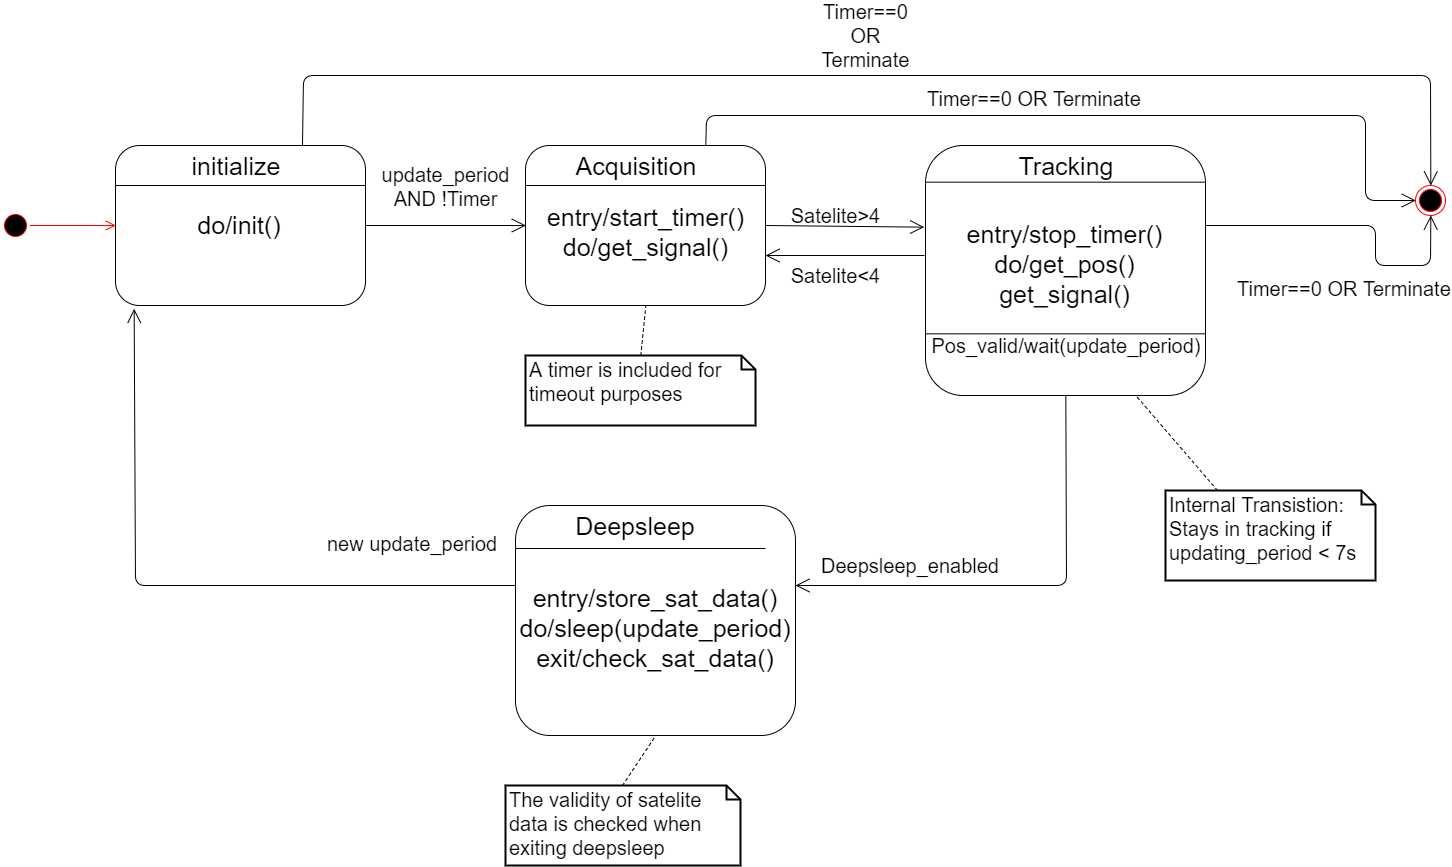
\includegraphics[width=15 cm]{Project_Report/Images/Energymodel.png}
\caption{The state diagram which represent the energy model}
\label{fig:GPS energymodel}
\end{figure}

\section{The model}
We can derive a prediction of the energy cost of acquiring a fix, by using the state diagram from \ref{fig:GPS energymodel}. The prediction will highlight which update period that is beneficial for having an optimal energy strategy. 
 
The Python script in appendix \ref{Appendix:make_energy_model.py} use the method that is derived in this subsection to predict the energy consumption over a range of update periods and durations. An update period is defined as the time from the microcontroller sends a positional request until the next request. The energy consumption over an update period is:
\begin{equation}
E_{period} = P_{period}*T_{period}
\end{equation}
\label{equation:general}
During an update period, the microcontroller transitions between the states in figure \ref{fig:GPS energymodel}. The total energy consumption $E_{fixperiod}$ can therefore be written as the sum of the energy of each state:

\begin{equation}
E_{period} = P_{Initialize}*T_{Initialize} + P_{Acquisition}*T_{Acquisition} + P_{Tracking}*T_{Tracking} + P_{Deepsleep}*T_{Deepsleep}
\end{equation}
\label{equation:energyperiod}

If the microcontroller is kept in tracking state, the initial energy used in initialize, acquisition and deepsleep is omitted. We omit the initial energy used in initialize and acquisition for the first fix during an update period of 1 \,s, because it becomes insignificant over a long duration. 
\begin{equation}
E_{Period = 1 \,s} = P_{Tracking}*T_{Tracking}
\end{equation}
\label{equation:1s}


The time used in deepsleep during an update period is dependent on the overhead of waking the microcontroller from deepsleep and acquiring a fix:

\begin{equation}
T_{Deepsleep} = T_{Updateperiod} - T_{Initialize} - T_{Acquisition} - T_{Tracking}
\end{equation}
\label{equation:energydeepsleep}
$T_ {Acquisition}$ depends on the validity of satellite data which is given by the update period. The total energy consumption over a duration t is given by the energy consumption of a fix period multiplied by the number of periods during the total duration t:

\begin{equation}
 E_{total} = E_{Updateperiod}* \frac{t}{Updateperiod}
\end{equation}
\label{equation:energytotal}

 We can use the average values from the previous subsection to calculate the power consumption for each state. This is shown in table  \ref{Table:data for the energy model}. The power is also plotted in a pie diagram in figure \ref{fig:powerconsumption}
\begin{table}[h!]
\begin{center}
 \begin{tabular}{||c c||} 
 \hline
  State &  Power(W) \\ [0.5ex] 
 \hline\hline
  Initialize & 0.32099 \\ 
 \hline
 Acquisition & 0.2576 \\
 \hline
 Tracking & 0.2324 \\
 \hline
 Deepsleep & 0.0105 \\
 [1ex]
 \hline
\end{tabular}
\end{center}
\caption{Power consumption of each state}
\label{Table:data for the energy model}
\end{table}

\begin{figure}[H]
\centering
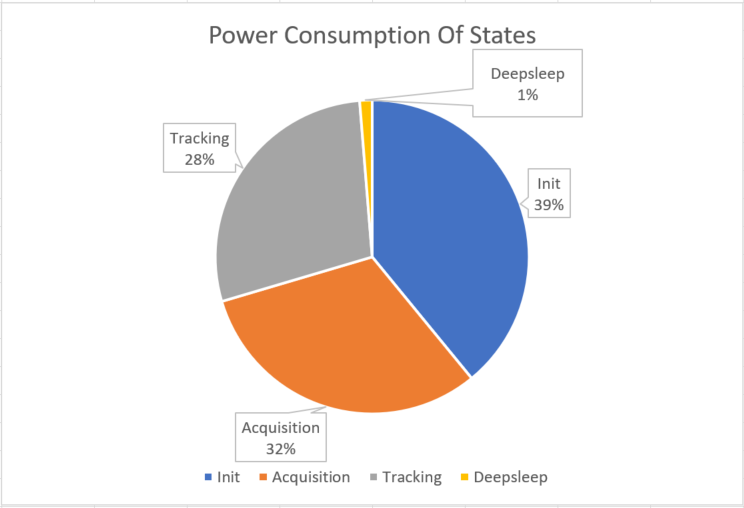
\includegraphics[height=7.5cm]{Project_Report/Images/Power.PNG}
\caption{The pie diagram of the power in table \ref{Table:data for the energy model}}
\label{fig:powerconsumption}
\end{figure}

The pie diagram shows how the majority of the power is associated with the initializing of the microcontroller. The second biggest contribution to power consumption is the acquisition state, followed by the tracking state. The power consumption in deepsleep is insignificant compared to the other states, which further encourage the use of deepsleep as a power saving strategy. The energy consumption over 1 year with a range of update periods included in table \ref{Table:data for the energy model}. The table is derived by using equation 6.5


\begin{table}[h!]
\begin{center}
 \begin{tabular}{||c c||} 
 \hline
 Energy Consumption & \\
 \hline
  Update Period & Duration = 1 year \\[0.5ex] 
 \hline\hline
  1 \,s & 7329470.97 \,J \\ 
 \hline
  7 \,s & 9485627.84 \,J \\
  \hline
  8 \,s & 8341511.51 \,J \\
  \hline
  9 \,s & 7451643.26 \,J \\
  \hline
  10 \,s & 6739748.65 \,J \\
 \hline
  60 \,s & 1400539.13 \,J \\
 \hline
  1800 \,s & 368291.96 \,J \\
  \hline
  3600 \,s & 350494.59 \,J \\
  \hline
  14399 \,s & 337146.88 \,J \\
  \hline
  14400 \,s & 352836.73 \,J \\
  \hline
  15551700 \,s & 332715.87 \,J \\
  \hline
  15552000 \,s & 332718.38 \,J \\[1ex]
 \hline
\end{tabular}
\end{center}
\caption{Table displaying the energy consumption over different durations and update periods}
\label{Table:energy}
\end{table}


\section{Energy Analysis}

The pie diagram from \ref{fig:powerconsumption} doesn't identify the energy demand of each state. The energy consumption of a state depends on the time that it's active. We know from equation 6.5 that it's only the time used in acquisition and deepsleep that varies. All the other times in our model is static. The time used in acquisition is an important factor for energy consumption. As explained in the theory chapter, the receiver can be in of three scenarios: 

\begin{itemize}
    \item Valid Ephemeris \& valid Almanac: Time used in acquisition: 1\,s. This is the scenario when the update period is in the range [1,14399]\,s. This scenario is equal to a Hot start.
    \item Invalid Ephemeris \& valid Almanac: Time used in acquisition: 30\,s. This is the scenario when the update period is in the range [14400,15551700]\,s. This scenario is equal to a Warm start.
    \item Invalid Ephemeris \& invalid Almanac: Time used in acquisition: 35\,s. This is the scenario when the update period is in the range [15551700, $\infty$ ]\,s. This scenario is equal to a Cold start.
\end{itemize}

We suspect that the energy consumption of each state will vary for each scenario, since the time in acquisition state varies. 

\subsection{Valid Ephemeris \& valid Almanac}

Figure \ref{fig:firstcase} shows the energy consumption over a duration of 1 year when the update period is 14399 \,s. The pie diagram shows the contribution from each state to the energy consumption. 

\begin{figure}[H]
\centering
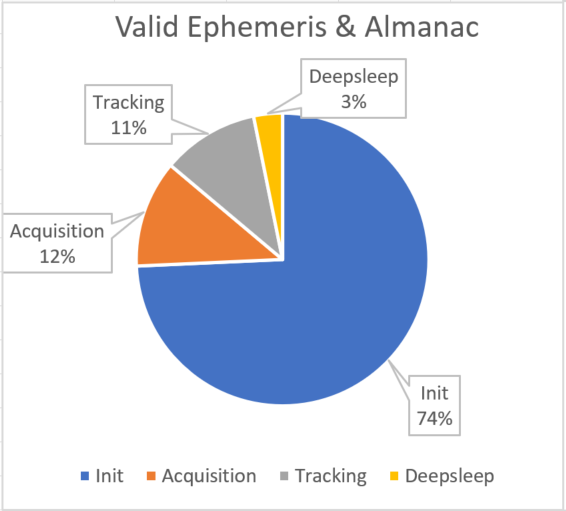
\includegraphics[height=7.5cm]{Project_Report/Images/Allvalid.PNG}
\caption{The energy consumption over 1 year with an update period of 14399 seconds}
\label{fig:firstcase}
\end{figure}

The GPS receiver uses only 1 \,s in the acquisition state because of the validity of the satellite data. This makes the initializing state, the main factor for the energy consumption. The receiver spends a small amount of time in deepsleep because of the high update frequency. This makes the deepsleep an insignificant contributor to the energy consumption. 

\subsection{Invalid Ephemeris \& valid Almanac}
Figure \ref{fig:secondcase} shows the energy contribution over 1 year for each state when the update period is 14400 \,s. An update period of [14400,15551700] \,s will make the Ephemeris invalid.

\begin{figure}[H]
\centering
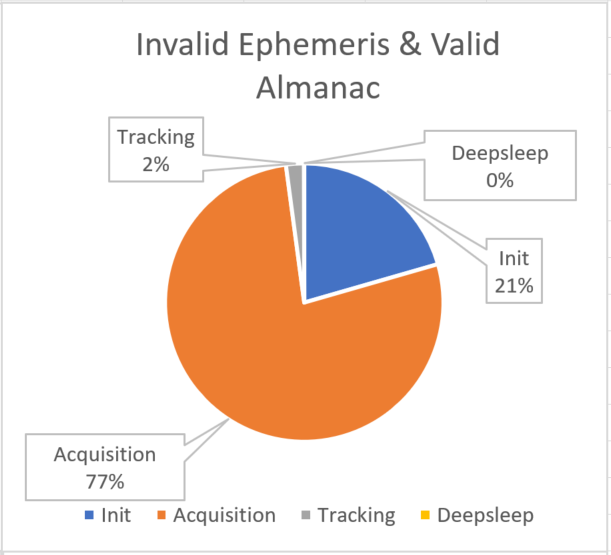
\includegraphics[height=7.5cm]{Project_Report/Images/invalidvalid.PNG}
\caption{The energy consumption over 1 year with an update period of 14400 seconds}
\label{fig:secondcase}
\end{figure}

Comparing figure \ref{fig:firstcase} with figure \ref{fig:secondcase}, we can see that the major energy consumer isn't the initialization state but the acquisition state. This is because of the added time penalty of waiting 30 \,s instead of 1 \,s in acquisition state. The added time penalty comes from time used in acquisition to download a valid Ephemeris. The update frequency is high, which makes the receiver spend a small time in deepsleep. This makes deepsleep a small part of the energy consumption.  

\subsection{Invalid Ephemeris \& invalid Almanac}

The energy consumption of each state when both the Ephemeris and Almanac is invalid is show in figure \ref{fig:thirdcase}.

\begin{figure}[H]
\centering
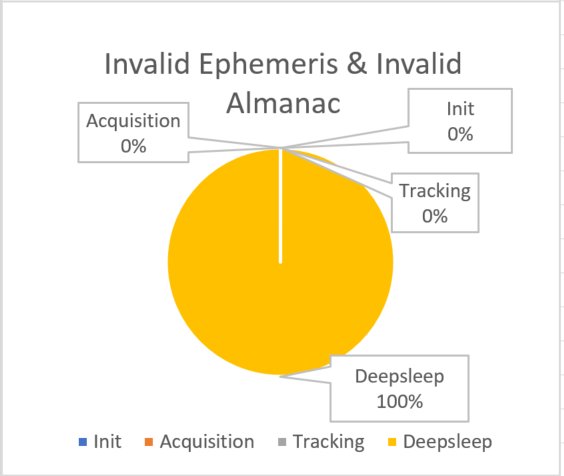
\includegraphics[height=7.5cm]{Project_Report/Images/invalidinvalid.PNG}
\caption{The energy consumption over 1 year with an update period of 15551700 seconds}
\label{fig:thirdcase}
\end{figure}

 Both the Ephemeris and Almanac is invalid when an update period of 15551700 \,s (180 days) is used. The receiver has to spend 35 \,s in the acquisition state to download the valid satellite data. The pie diagram in figure \ref{fig:thirdcase} is different from figure \ref{fig:firstcase} and figure \ref{fig:secondcase}, in that the major energy consumption is from deepsleep. This is because of the low update frequency which cause the system to spend the majority of its time in deepsleep. A longer update period will therefore use less energy but give a coarser positional fix over a specific duration. 

\newpage
\chapter{Discussion and Conclusion}
Table \ref{Table:energy} from the previous chapter is plotted in figure \ref{fig:energyconsumption}. The plot shows the energy consumption for various update periods over a duration of 1 year.

\begin{figure}[H]
\centering
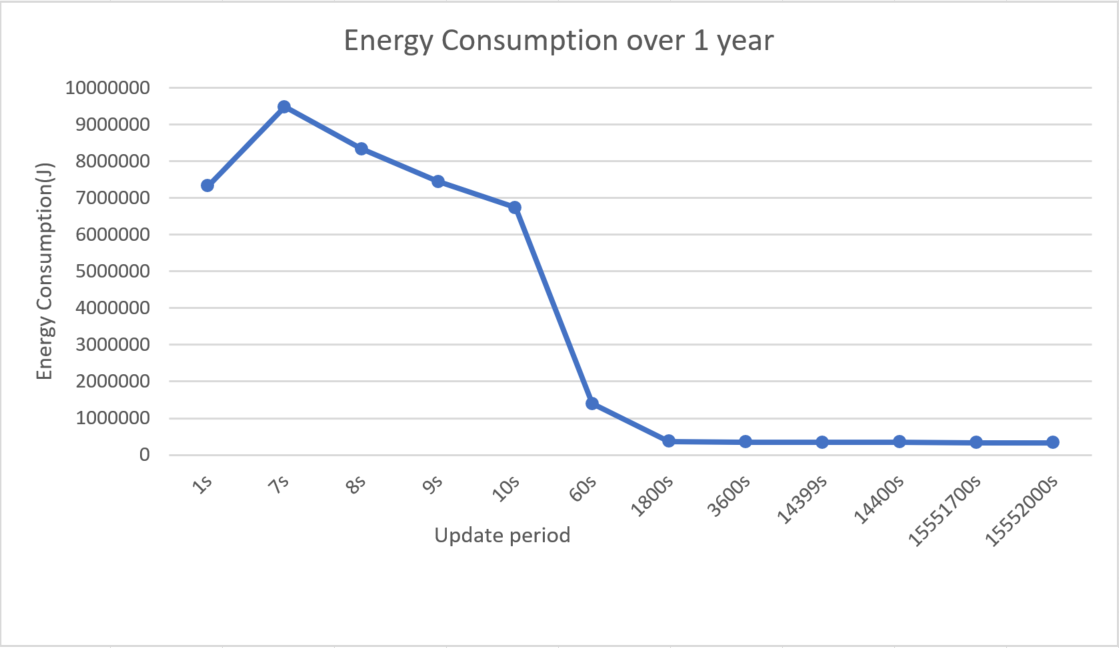
\includegraphics[height=9.0cm]{Project_Report/Images/energyconsumption.PNG}
\caption{The plot of the energy model from table \ref{Table:energy}}
\label{fig:energyconsumption}
\end{figure}

The plot shows that the energy consumption increases when the update period is increased from 1 second to 7 seconds. This may not be intuitive as the increased update period will cause the system to spend a longer time in deepsleep. The increased energy consumption is caused by the overhead of waking up the system from deepsleep, initializing it and acquiring a fix in acquisition. From figure \ref{fig:firstcase}, we know that the initializing state is a major contributor to energy consumption. An update period that is bigger than  1 second forces the system to repeat this cycle multiple times instead of staying in the tracking state. An update period between (1,7) which uses deepsleep, is not possible because the overhead uses 6 seconds.

The energy consumption decreases when the update period is increased from 7 \,s. At an update period of 9 \,s, the energy consumption is still higher then an update period of 1 \,s. But by 10 \,s , the energy consumption is less then at 1 \,s. This means that because of the added overhead, it is always more beneficial to use an update period of 1 \,s which continuously stays in tracking state instead of using an update period in the range [7,9] \,s. The initial assumption that deepsleep is always a preferred method is therefore inaccurate. 

The energy consumption continues to decrease until the update period is 14399 \,s. After the update period is increased from 14399 \,s, the energy consumption starts to increase. This is shown in table \ref{Table:data for the energy model}. We know from the previous chapter, that an update period that is longer than 14399 \,s will make the Ephemeris invalid. The pie diagram in figure \ref{fig:secondcase} shows how the acquisition state will be the major energy consumer. The addition of the time penalty in acquisition will cause an increase in energy consumption. The time penalty is due to the invalidity of the Ephemeris .By using algorithm in \ref{code:limit}, we find the range of update periods where it's optimal to use an update period of 14399 \,s instead. Algorithm \ref{code:limit} returns 14401 \,s as the limit. This means that because of the invalidity of the Ephemeris, it's better to use an update period of 14399 instead of 14400 \,s or 14401 \,s. From table \ref{Table:energy} we see that the difference in energy consumption over a year from an update period of 14399 \,s to 14400 \,s is:
\begin{equation}
352836.7334 J - 337146.8816 J = 15689.9174 J
\end{equation}

This shows that according to the model, it's optimal to use an update period that preserves the validity of the Ephemeris and Almanac by having an update period that is slightly less than 14400 \,s, instead of having an update period of 14400 \,s or slightly more.  


\lstset{language=Python}          % Set your language (you can change the language for each code-block optionally)
\begin{lstlisting}[frame=single, caption= Code used for finding the beneficial limit]  % Start your code-block

    optimal   =   Energy_consumption[4][5]
    temp     =   Energy_consumption[4][6]
    fix_o = 14400

    while(optimal<temp):  
        T_sleep = fix_o - T_wake - 30 - T_track
        optimal = (P_sleep*T_sleep + P_wake*T_wake + P_acq*30 + P_track*T_track)*t[4]/fix_o
        fix_o = fix_o + 1
    print("fix_o",fix_o)

\end{lstlisting}
\label{code:limit}


The plot from \ref{fig:energyconsumption} continues to decrease until the updated period is increased to 15551700 \,s. The energy consumption increases after this point. An update period over 15551700 \,s causes the Almanac to be invalid. This means that the system will spend 35 \,s instead of 30 \,s in acquisition state to download the satellite data. The plot in \ref{fig:energyconsumption} shows that the increased energy consumption is insignificant. This is highlighted by table \ref{Table:energy}, which shows a difference of less than 1 J between an update period of 15551700 \,s and 15552000 \,s. The small difference in energy consumption is because of the small penalty of 5 \,s that is added to download a valid Almanac.  Most IoT applications need an update frequency that is higher than 180 days, which makes an update period in the range of [57080, 5551700 ] \,s impractical. 

In the introduction chapter, we explained the necessity for an energy model for controlling a GPS optimally. This project has explained how the simple model in figure \ref{fig:energyconsumption} can be used by an application to determine the optimal energy strategy for requesting a positional fix. For instance, if an application wants a fix every 8 second, it can use the model to predict that it is better to have an update period of 1 second. Alternatively, the application can decide that the energy cost isn't worth the positional fix. 

The time limit of the project compelled us to make a simple model. The consequence of the simple model is that the assumptions might be too oversimplified. The oversimplified model, gives an oversimplified prediction. The assumption that the receiver will use the specified time in acquisition is certainly not always the case. The time used in acquisition is dependent on signal strength, and not including the environment that the receiver operates in, is therefore a crucial oversimplification of the model. Further work should therefore include a probability of the predicted time in acquisition. 

The state diagram from figure \ref{fig:GPS reciever} should also be extended with states that receiver transitions to if it doesn't acquire a fix within the timeout. A failure of acquiring a fix, might require a different strategy as it could inform the application that the receiver is in an environment where signal strength is low. For example a valley or under a tunnel. 

Future work should also establish energy saving techniques that are specific for a certain state and update period. The comparison between the pie diagrams from the Energy modeling chapter, shows that there is different energy requirement for the states for different update periods. The initialize state is a major energy factor when satellite data is valid. Specific methods should therefore be used for decreasing the energy consumption when a low update period is used. Contrarily, when a greater update period is used, the acquisition is the main energy consumer. This project highlights that there are considerable benefits in using the simple energy model for an optimal energy strategy, despite the simplified model. 



% Bibliography - edit references.bib and use the \cite command in text
\bibliographystyle{plain}
\bibliography{Content/references.bib}
\begin{appendices}
\chapter{C027.cpp}
\begin{lstlisting}
#include "mbed.h"
#include "C027.h"
#include "rtos.h"

int power= 0;
char order= 'O';
int BAUDRATE=9600;
int timer;
int MEASURE_TIME= 1000000000;
C027 devkit;
DigitalOut trigger(D0);

void serialhandler(){
    //devkit.gpsPower(true);
    
    // open the gps serial port
    Serial gps(GPSTXD, GPSRXD);
    gps.baud(BAUDRATE);
    
    // open the PC serial port and (use the same baudrate)
    Serial pc(USBTX, USBRX);
    pc.baud(BAUDRATE);
    //devkit.gpsPower(true);
    while(1){
        if(pc.readable()){
            order = pc.getc();
            if(order=='D' && power){
                devkit.gpsPower(false);
                timer= MEASURE_TIME;
                power = 0;
                }
            else if(order=='E' && !power){
                devkit.gpsPower(true);
                timer= MEASURE_TIME;
                power= 1;
                }
            else if(order=='R'){
                    devkit.gpsReset();
                    timer = 0;
                    }  
        }
    if(gps.readable() && pc.writeable()){
        pc.putc(gps.getc());
        }
    }
}
void measure(){
     while(1){
     trigger.write(1);
     wait_ms(10);
     trigger.write(0); //Trekker utgangen ned
     wait_ms(10);
     timer --;
     while(timer<=0){
         wait_ms(1);
         }
    }
}
int main(){
    devkit.gpsPower(false);
    Thread thread_serial;
    Thread thread_measure;
    
    thread_measure.start(measure);
    thread_serial.start(serialhandler);
   while(1){}
    return 0; }
\end{lstlisting}
\label{Appendix:C027.Cpp}


\chapter{L76GNSS.py}
\begin{lstlisting}
from machine import Timer
import time
import gc
import binascii

class L76GNSS:
    STANDBY = bytes( [0x24,0x50,0x4D,0x54,0x4B,0x31,0x36,0x31,0x2C,0x30
    ,0x2A,0x32,0x38,0xD,0xA])
    GLONASS = bytes( [0x24,0x50,0x4D,0x54,0x4B,0x33,0x35,0x33,0x2C,
    0x30,0x2C,0x31,0x2A,0x33,0x36,0xD,0xA]) 
    COLD_START = bytes( [0x24,0x50,0x4D,0x54,0x4B,0x31,0x30,0x34,0x2A,
    0x33,0x37,0xD,0xA])
    PERIODIC_MODE = bytes( [0x24,0x50,0x4D,0x54,0x4B,0x32,0x32,0x35,
    0x2C,0x32,0x2C,0x33,0x30,0x30,0x30,0x2C,0x31,0x32,
    0x30,0x30,0x30,0x2C,0x31,0x38,0x30,0x30,0x30,0x2C,
    0x37,0x32,0x30,0x30,0x30,0x2A,0x31,0x35])

    GPS_I2CADDR = const(0x10)

    def __init__(self, pytrack=None, sda='P22', scl='P21', timeout=None):
        if pytrack is not None:
            self.i2c = pytrack.i2c
        else:
            from machine import I2C
            self.i2c = I2C(0, mode=I2C.MASTER, pins=(sda, scl))

        self.chrono = Timer.Chrono()

        self.timeout = timeout
        self.timeout_status = True

        self.reg = bytearray(1)
        self.i2c.writeto(GPS_I2CADDR, self.reg)
        self.fix = 0
        self.first_fix=0
        self.timestamp= 0
        self.gpgga_s= ''

        self.lat_d = 0
        self.lon_d = 0

    def write_gps(self,data,wait=True):
        print(data)
        self.i2c.writeto(GPS_I2CADDR, data)
        if wait:
             self.wait_gps()    
    def wait_gps(self):
        count = 0
        time.sleep_us(10)
        while self.i2c.readfrom(GPS_I2CADDR, 1)[0] != 0xFF:
            time.sleep_us(100)
            count += 1
            if (count > 500):  # timeout after 50ms
                raise Exception('Pytrack board timeout')


           
    def _read(self):
        self.reg = self.i2c.readfrom(GPS_I2CADDR, 64)
        return self.reg
    def _set_time(self):
        print('_set_time')
        self.timestamp = self.gpgga_s[1]
        print('timestamp set',self.timestamp)

    def _convert_coords(self):
        lat = self.gpgga_s[1]
        lat_d = (float(lat) // 100) + ((float(lat) % 100) / 60)
        lon = self.gpgga_s[3]
        lon_d = (float(lon) // 100) + ((float(lon) % 100) / 60)
        if self.gpgga_s[2] == 'S':
            lat_d *= -1
        if self.gpgga_s[4] == 'W':
            lon_d *= -1
        return(lat_d, lon_d)

    def get_fix(self):
        temp_fix= self.gpgga_s[6]
        self.fix = int(temp_fix)

    def coordinates(self, debug=False):
        lat_d, lon_d, debug_timeout = None, None, False
        if self.timeout != None:
            self.chrono.reset()
            self.chrono.start()
        nmea = b''
        while True:
            if self.timeout != None and self.chrono.read() 
            >= self.timeout:
                self.chrono.stop()
                chrono_timeout = self.chrono.read()
                self.chrono.reset()
                self.timeout_status = False
                debug_timeout = True
            if self.timeout_status != True:
                gc.collect()
                break
            nmea += self._read().lstrip(b'\n\n').rstrip(b'\n\n')
            gpgga_idx = nmea.find(b'GPGGA')
            if gpgga_idx >= 0:
                gpgga = nmea[gpgga_idx:]
                e_idx = gpgga.find(b'\r\n')
                if e_idx >= 0:
                    try:
                        gpgga = gpgga[:e_idx].decode('ascii')
                        print (gpgga)
                        self.gpgga_s = gpgga.split(',')
                        print(self.gpgga_s)
                        self.get_fix()
                        if(self.fix >0):
                            self.lat_d, self.lon_d = self
                            ._convert_coords(self.gpgga_s)
                    except Exception:
                        pass
                    finally:
                        nmea = nmea[(gpgga_idx + e_idx):]
                        gc.collect()
                        break
            else:
                gc.collect()
                if len(nmea) > 4096:
                    nmea = b''
           # time.sleep(0.1)
        self.timeout_status = True
        if debug and debug_timeout:
            print('GPS timed out after %f seconds' % (chrono_timeout))
            return(None, None)
        else:
            return(lat_d, lon_d)


\end{lstlisting}
\label{Appendix:L76GNSS.py}
\end{appendices}




\end{document}
